\chapter{SYSTEM DESIGN AND IMPLEMENTATION}

This chapter describes the implementation of the system which consists of: A social media website, an image processing module, a video processing module, a database. In \textit{System overview and requirement analysis} section, everything is briefly described as a whole. In other sections, structure and details of each component are defined more comprehensively.
\section{System overview and requirement analysis}

\subsection{System overview}
Figure \ref{chap3:system_overview_basic} shows a concise overview of how the system operates. Users interact with the website through front-end. The input of users can come in the form of images, videos or label contribution. Back-end receives input and stores in the database. Concurrently, inputs are sent to image processing module/video processing module . Outputs from analysis server are sent back to back-end and then stored in database. The back-end is also responsible for obtaining appropriate contents from the database to display to users through front-end.

\begin{center}
    \begin{figure}[H]
    \centering
    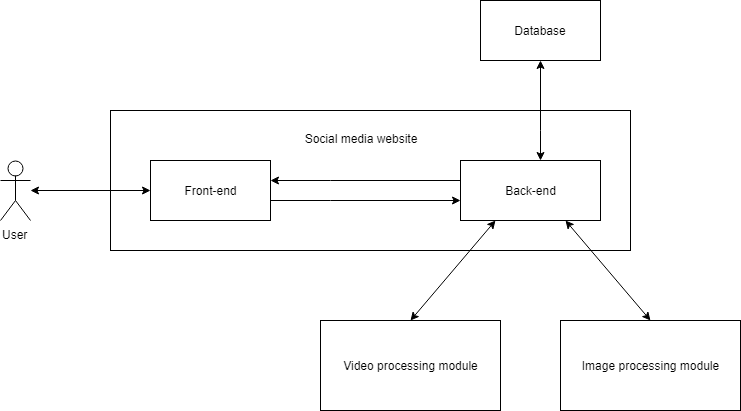
\includegraphics[width=1\columnwidth]{images/chap3/system_overview_basic.png}
    \caption{An overview of the system}
    \label{chap3:system_overview_basic}
    \end{figure}
\end{center}
\subsection{Requirement analysis}
A requirements analysis is essential to any system. In this section, this thesis defines functional as well as non-function requirements for the system. Use cases and a system overview is also outlined in the following subsections.
\subsubsection{Types of users}
As with any sophisticated system, the proposed system has many types of user. Those type of users are:

\begin{itemize}
    \item \textbf{Guest users}: Users that have not verify their account by authentication methods.
    \item \textbf{Verified users}: Users that are verified with the system by authentication methods.
    \item \textbf{Admins}: Supervisors of the system. This title is given to people who are responsible for managing the system.
\end{itemize}
\subsubsection{Functional Requirements}
As stated in \ref{chap:solution}, this project would build a social media website for security. Such a website must have functions of a typical social media as well as additional functions for security. Those functions would include:
\begin{itemize}	
    \item Verified users and Guest users can view posts by other users. 
    \item Verified users could create posts with images or videos and includes location and time information in their posts. The website stores posts and image/videos in databases and analyze them through analyzing modules.
    \item Verified users could contribute to the system by labeling videos. Labels of videos are stored in the database and are used to train video classification modules.
    \item Verified users could subscribe to a location to get notifications about the suspicious videos from that location.
    \item When suspicious videos are detected, notifications are sent to Users subscribed to nearby locations.
    \item The system can recognize faces from images and logs their occurrences to the database.
\end{itemize}


\subsubsection{Non-functional Requirement}
In the scope of a thesis, the system has to acquire these requirements to perform processes that are stable and efficient for the user:
\begin{itemize}
	\item Reliability: The System is able to have 90\% uptime of Internet connection. It should have OAuth services via Google/Facebook(account kit) for authentication.
	\item Scalability: The website is able to handle many concurrent connections and manage a large amount of posts and store into NoSQL database .
	\item Usability: The website uses modern UI developed in HTML5. The user can use that UI easily to navigate between each page. It also has a fresh and well-designed interface for user to interact with
\end{itemize} 
\subsubsection{Use Cases}
\begin{center}
	\begin{figure}[H]
		\centering
		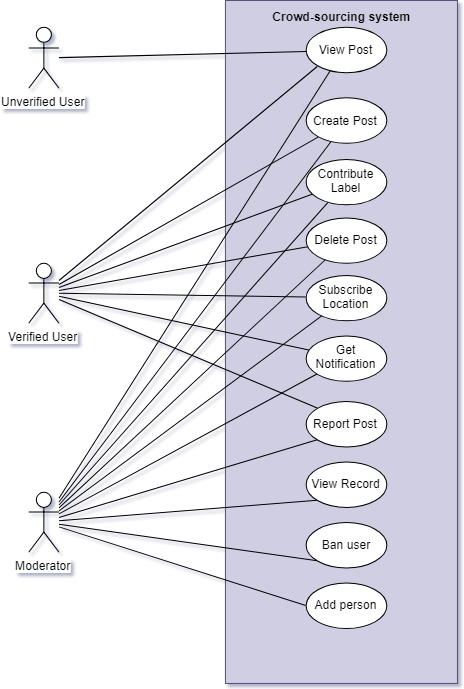
\includegraphics[width=0.75\columnwidth]{images/chap4/usecase.png}
		\caption{Use case diagram}
		\label{chap4:user_case_diagram}
	\end{figure}
\end{center}
% Please add the following required packages to your document preamble:
% \usepackage{multirow}
% Please add the following required packages to your document preamble:
% \usepackage{multirow}
% \usepackage[normalem]{ulem}
% \useunder{\uline}{\ul}{}
\begin{table}[]
\begin{tabular}{|P{5cm}|L{10cm}|}
		\hline
	Name							&   UC01 - Log in website     \\ \hline
	Description 	 				&   Users will be prompted to login with their account information before they can use the system.   \\ \hline
	Actor 							&  User and Moderator       \\ \hline
\multirow{3}{*}{Preconditions} 		&\tabitem The user has an website account \\ \
									&\tabitem The user is trying to log in with their account \\ \
									&\tabitem The user is not already logged in with website  \\ \hline
\multirow{2}{*}{Postconditions}	 	&\tabitem The user is logged in to the system     \\ 
									&\tabitem The user has access to the functions of the
									system\\ \hline
\multirow{9}{*}{Path} 				&\tabitem Primary path:    \\
									& 1.User accesses the URL \\ 
									& 1.1 The system prompts the user for their 
									account sign up. \\
									& 1.2 The user enters their username and
									password. \\
									& 1.3 The system authenticates the  login
									with website \\
									& 1.4 The user gains access to the systems
									functionality \\ \cline{2-2} 
									&\tabitem Alternate path  \\
									& 2. Invalid account user or banned \\
									& 2.1 User already logged in with website \\ \hline
	\end{tabular}
\end{table}
\begin{table}[]

	\begin{tabular}{|P{5cm}|L{10cm}|}
		\hline
		Name						&   UC02 - View all posts in website     \\ \hline
		Description 	 			&   Users can view detail in posts   \\ \hline
		Actor 						&  	User and Moderator       \\ \hline
		Preconditions 				& 	System check the role of the user to provide the following function 						 \\ \hline
		Postconditions	 			&							 \\ \hline 
\multirow{9}{*}{Path} 						&\tabitem Primary path:    \\
									& 1.Unverified-user press to title of the post \\ 
									& 1.1 The system inquire the user for their roles
									account . \\
									& 1.2 The user can see information of post and commend \\
									& 2. Verified-user and Moderator press to title of the post \\
									& 2.1 The system inquire the user for their roles
									account . \\
									& 2.2 Verified-user and Moderator can use feature as commend and report post \\ \cline{2-2} 
									&\tabitem Alternate path  \\
									& 3. View post by tab My Posts in Profile user\\ \hline
	\end{tabular}
\end{table}
\subsection{System overview}
Figure \ref{chap3:system_overview_basic} shows a concise overview of how the system operates. Users interact with the website through front-end. The input of users can come in the form of images, videos or label contribution. Back-end receives input and stores in the database. Concurrently, inputs are sent to analysis server . Outputs from analysis server are sent back to back-end and then stored in database. The back-end is also responsible for obtaining appropriate contents from the database to display to users through front-end.

\subsubsection{Main function of the system: Notify users about suspicious activity using data from posts.}

\begin{center}
	\begin{figure}[H]
		\centering
		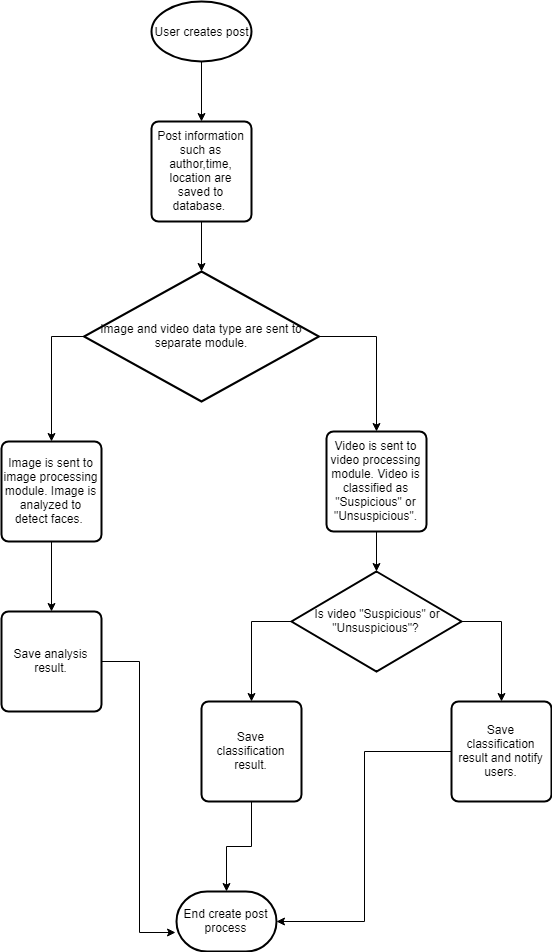
\includegraphics[width=0.7\columnwidth]{images/chap4/createpostflowchart.png}
		\caption{Create post flowchart.}
	\end{figure}
\end{center}

Specifically, users create post with image/video to provide data to back-end. Post also contains other information such as author, location, time. Back-end save all information from post and then deliver data to relevant module to analyze. When suspicious activity detected after analyzing, back-end notify users who subscribe to the exact location and users who subscribe to locations that are in a diameter of 1 kilometer from that location.

\section{Technologies}
\subsection{Node.js and Node Package Manager (npm)}
Node.js (Node) is a JavaScript runtime built on Chrome's V8 JavaScript engine (cite). Node supports executing JavaScript on server-side. Ryan Dahl was created Node.js in 2009. Node.js Foundation is in charge of the development of Node.js. After nine years since its release, the latest LTS version of Node.js is 10.14.2 (includes npm 6.4.1). “Node.js operates on a single thread, using non-blocking I/O calls, allowing it to support tens of thousands (cite) of concurrent connections held in the event loop.” Although JavaScript is single-threaded, thanks to the Event loop, Node.js can implement asynchronous I/O operations. The Event loop will transfer operations to the system kernel. “Since most modern kernels are multi-threaded, they can handle multiple operations executing in the background. When one of these operations completes, the kernel tells Node.js so that the appropriate callback may be added to the poll queue to executed eventually”. By utilizes non-blocking I/O, Node.js skips the waiting time for I/O calls, which is much higher than processing time.
\subsection{Keras}
Keras is a high-level framework for building Deep learning model build on top of Tensorflow or Theano library.\\
Keras provides APIs that are more friendly for new learner compared to Tensorflow. Besides that, Keras also has useful functions for preprocessing data.
\subsection{Gunicorn}
Gunicorn is a Python Web Server Gateway Interface (WSGI) HTTP server. A WSGI recieve requests from web servers and foward them to Python applications.
Gunicorn helps separating the operation between web servers and applications, making applications more portable. Moreover, Gunicorn provides features for deployment such as maximum of requests for each worker, number of workers, making it useful for this thesis.

\section{Database}
The project database divides into two different parts: \textbf{Cloud storage} for visual data such as image/video and a \textbf{NoSQL database} for other information. The primary target is to reduce website loading time. Let take an example, if files are stored directly on the back-end server. When many users request a file simultaneously, the server with limited bandwidth will cause delay. “53\% of mobile site visitors leave a page that takes longer than three seconds to load” – \href{https://think.storage.googleapis.com/docs/mobile-page-speed-new-industry-benchmarks.pdf}{Google}. If these files stored on cloud storage, the client will be served by the cloud storage provider, which has higher availability.
\subsection{Cloud storage}

\subsection{NoSQL database}
NoSQL databases were created in response to the limitations of traditional relational database technology. When compared against relational databases, NoSQL databases are more scalable and provide superior performance, and their data model addresses several shortcomings of the the relational model.

The advantages of NoSQL include being able to handle:

Large volumes of structured, semi-structured, and unstructured data
Agile sprints, quick iteration, and frequent code pushes
Object-oriented programming that is easy to use and flexible
Efficient, scale-out architecture instead of expensive, monolithic architecture
Hence, \textbf{MongoDB} is used to implement the database in this project
\subsubsection{Database overview}
Figure \ref{chap4:database_overview} displays the structure of the database which includes collections and relationships between them.
There are a total of 8 collections in the database: User, Visual data, Location, Notification, Person, Post, Record, Role. 
\begin{center}
	\begin{figure}[H]
		\centering
		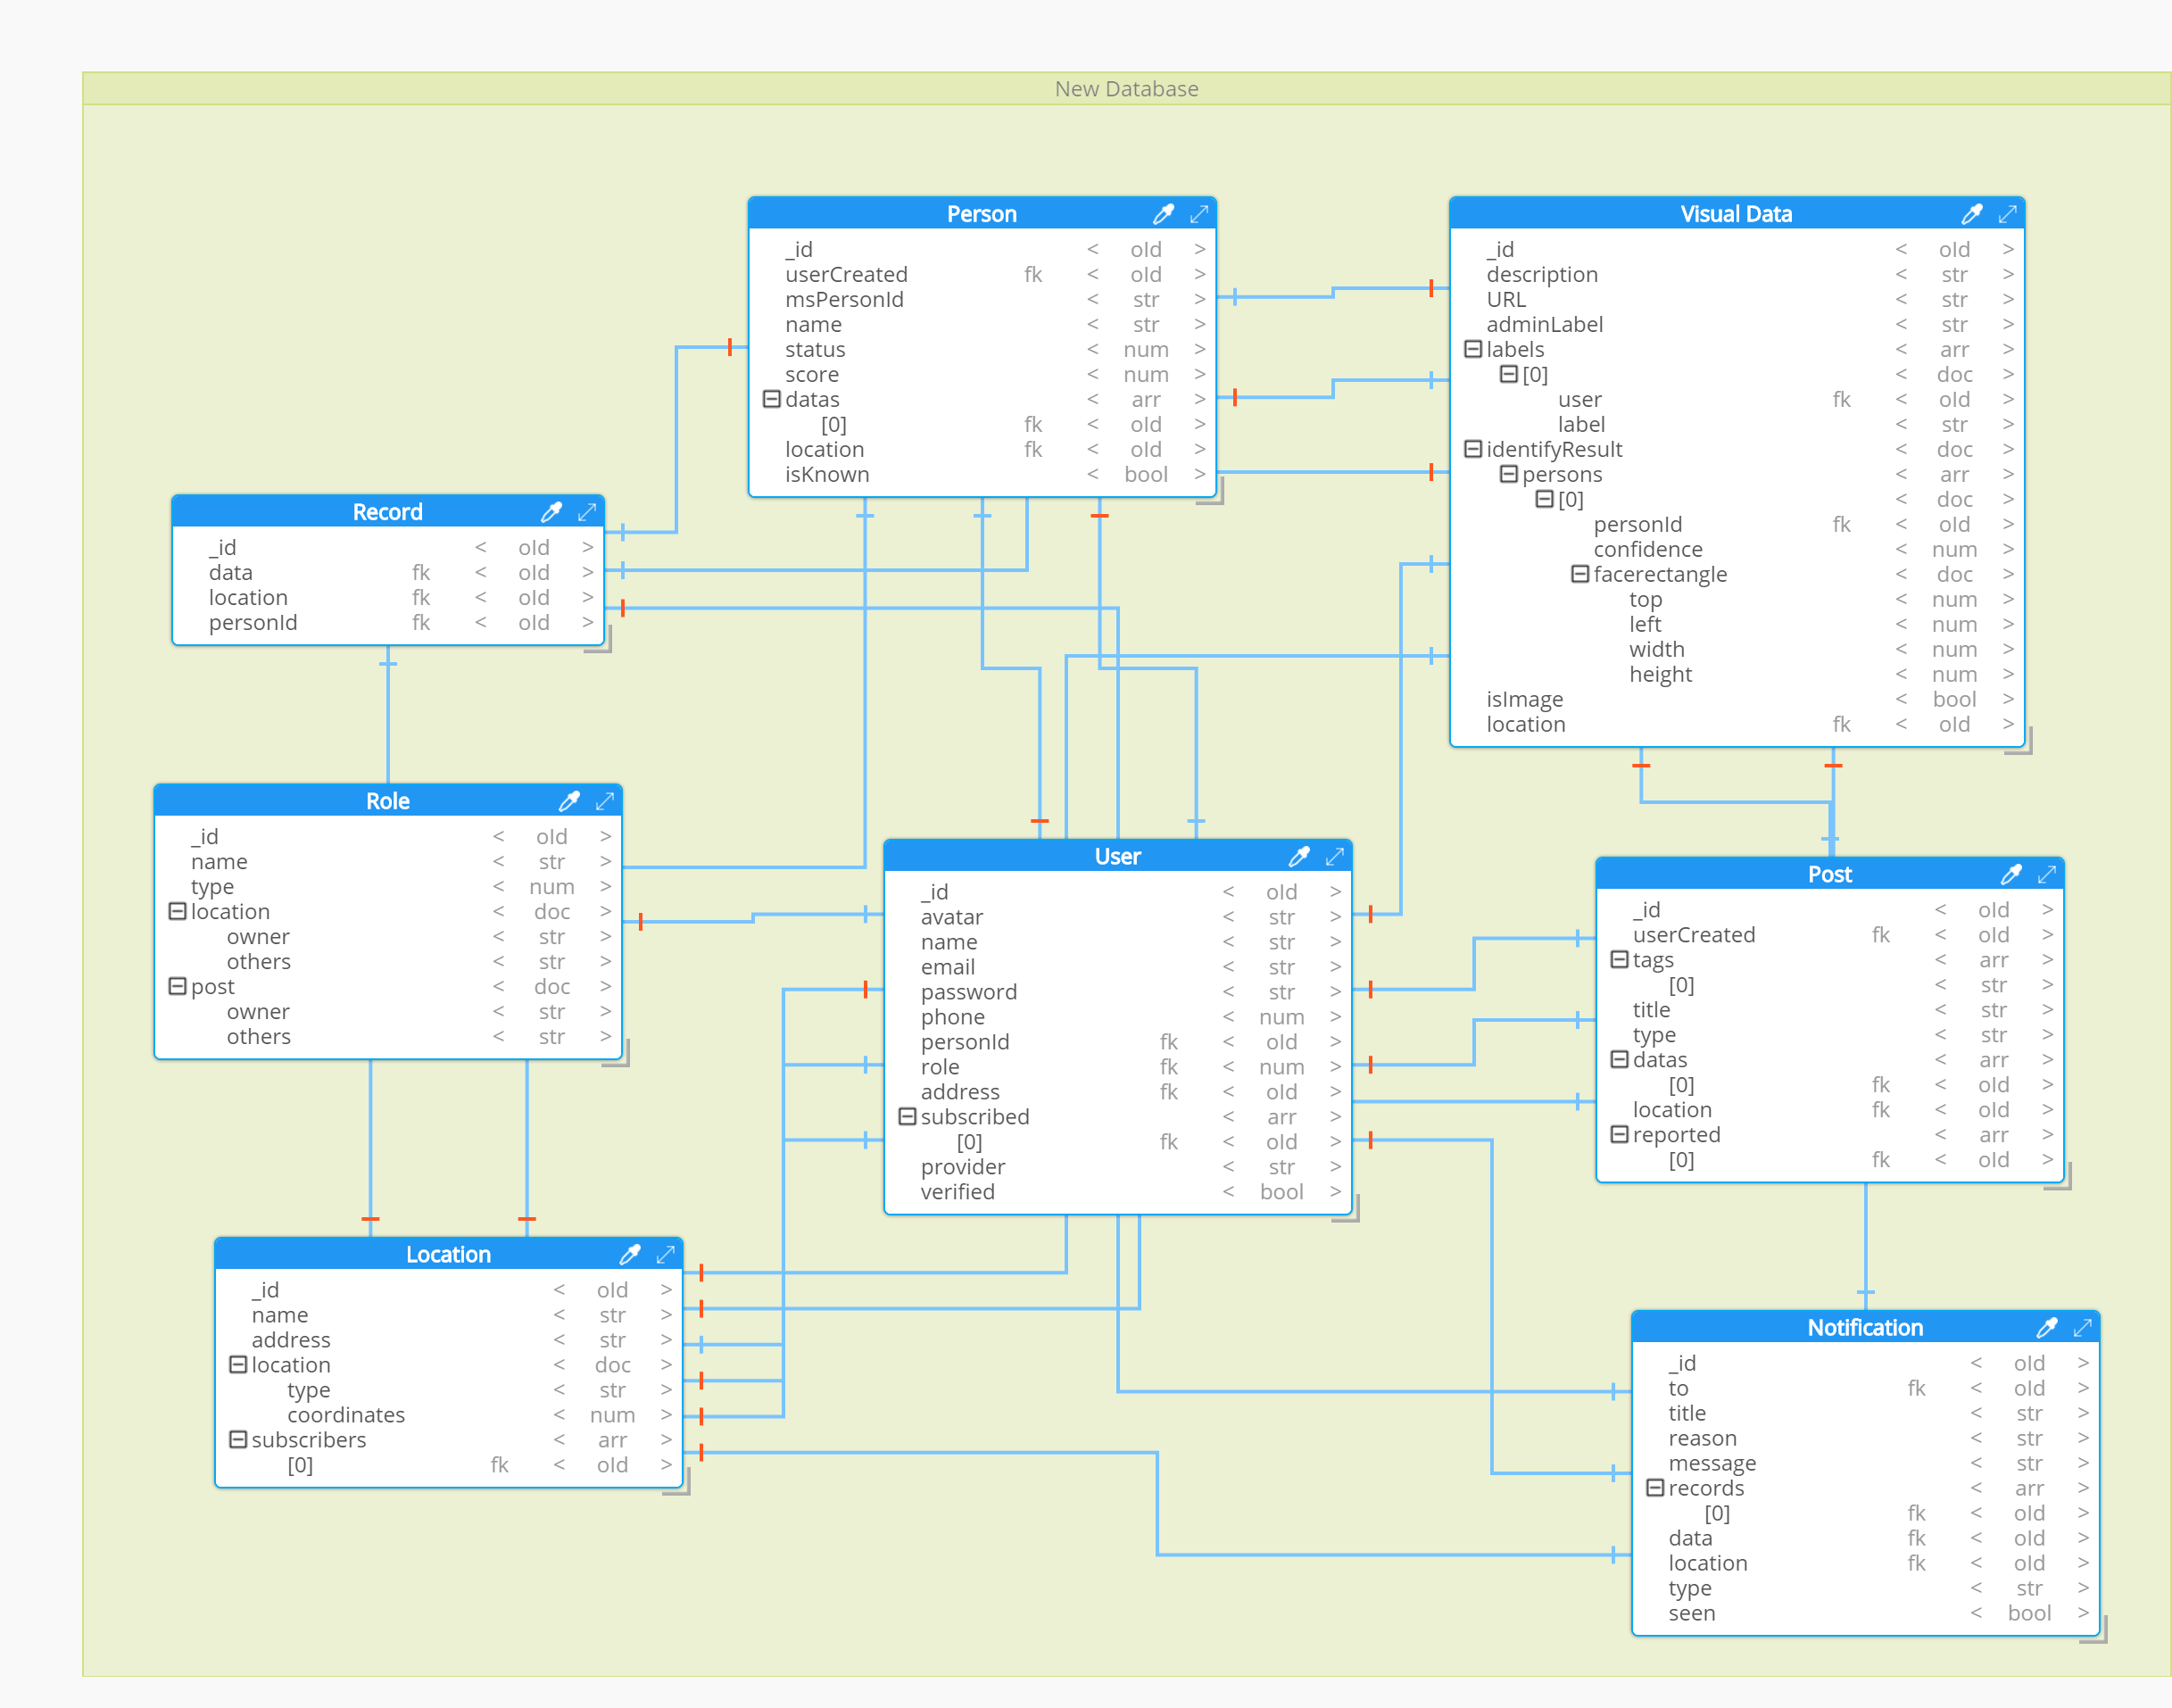
\includegraphics[width=1\columnwidth]{images/chap4/Model.png}
		\caption{An overview of the database}
		\label{chap4:database_overview}
	\end{figure}
\end{center}
\cleardoublepage
\subsubsection{Collections}
\textbf{User}
\begin{center}
	\begin{figure}[H]
		\centering
		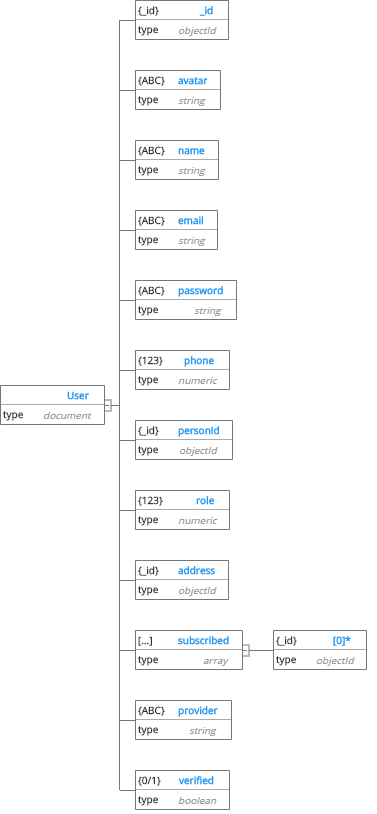
\includegraphics[width=0.5\columnwidth]{images/chap4/User.png}
		\caption{User collection}
	\end{figure}
\end{center}
\cleardoublepage
\textbf{Visual data}
\begin{center}
	\begin{figure}[H]
		\centering
		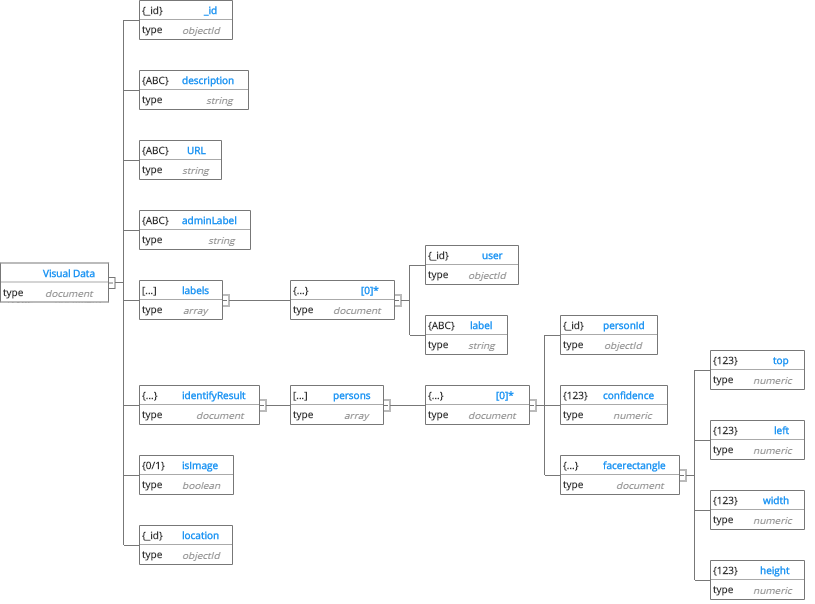
\includegraphics[width=1\columnwidth]{images/chap4/Visual.png}
		\caption{Visual Data collection}
	\end{figure}
\end{center}
\cleardoublepage
\textbf{Location}
\begin{center}
	\begin{figure}[H]
		\centering
		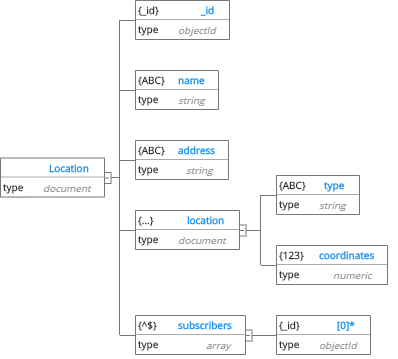
\includegraphics[width=1\columnwidth]{images/chap4/Location.png}
		\caption{Location collection}
	\end{figure}
\end{center}
\cleardoublepage
\textbf{Notification}
\begin{center}
	\begin{figure}[H]
		\centering
		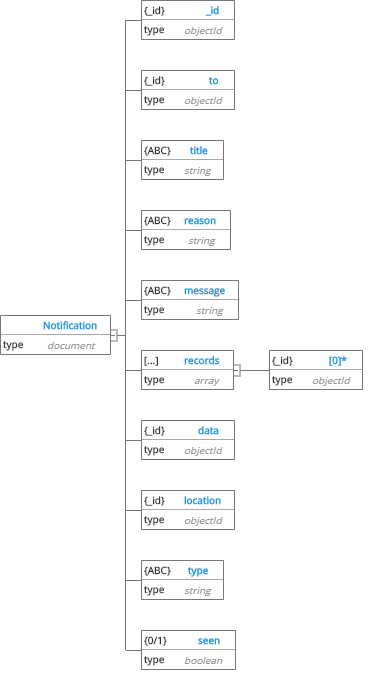
\includegraphics[width=0.7\columnwidth]{images/chap4/Notification.png}
		\caption{Notification collection}
	\end{figure}
\end{center}
\cleardoublepage
\textbf{Person}
\begin{center}
	\begin{figure}[H]
		\centering
		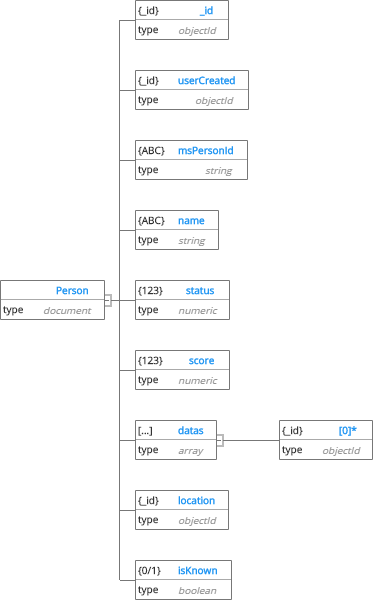
\includegraphics[width=0.7\columnwidth]{images/chap4/Person.png}
		\caption{Person collection}
	\end{figure}
\end{center}
\cleardoublepage
\textbf{Post}
\begin{center}
	\begin{figure}[H]
		\centering
		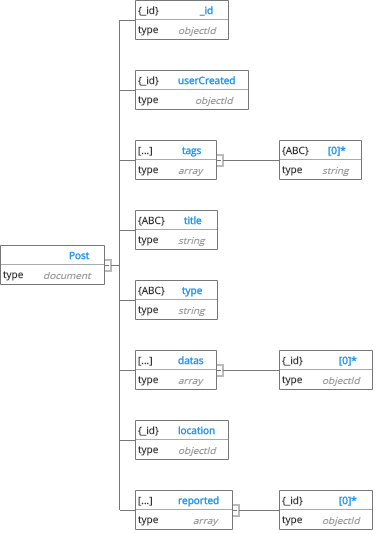
\includegraphics[width=0.7\columnwidth]{images/chap4/Post.png}
		\caption{Post collection}
	\end{figure}
\end{center}
\cleardoublepage
\textbf{Record}
\begin{center}
	\begin{figure}[H]
		\centering
		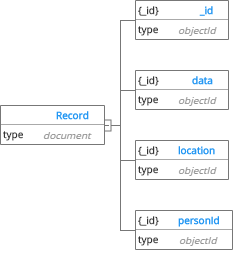
\includegraphics[width=0.7\columnwidth]{images/chap4/Record.png}
		\caption{Record collection}
	\end{figure}
\end{center}
\cleardoublepage
\textbf{Role}
\begin{center}
	\begin{figure}[H]
		\centering
		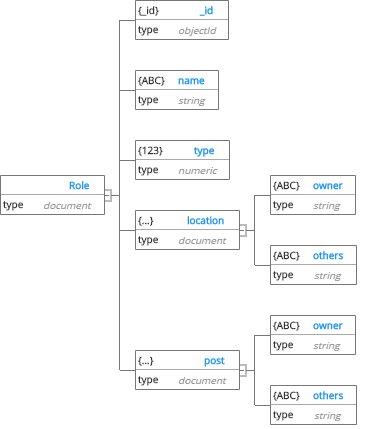
\includegraphics[width=0.7\columnwidth]{images/chap4/Role.png}
		\caption{Role collection}
	\end{figure}
\end{center}
\cleardoublepage
\subsubsection{Relationships}
\begin{table}[H]
	\begin{tabular}{|l|l|}
		\hline
		\textbf{Children field}                             & \textbf{Parent field} \\ \hline
		Location.subscribers.{[}0{]}                        & User.\_id             \\ \hline
		Notification.to                                     & User.\_id             \\ \hline
		Notification.records.{[}0{]}                        & Record.\_id           \\ \hline
		Notification.data                                   & Visual Data.\_id      \\ \hline
		Notification.location                               & Location.\_id         \\ \hline
		Person.userCreated                                  & User.\_id             \\ \hline
		Person.datas.{[}0{]}                                & Visual Data.\_id      \\ \hline
		Person.location                                     & Location.\_id         \\ \hline
		Post.userCreated                                    & User.\_id             \\ \hline
		Post.datas.{[}0{]}                                  & Visual Data.\_id      \\ \hline
		Post.location                                       & Location.\_id         \\ \hline
		Post.reported.{[}0{]}                               & User.\_id             \\ \hline
		Record.data                                         & Visual data.\_id      \\ \hline
		Record.location                                     & Location.\_id         \\ \hline
		Record.personId                                     & Person.\_id           \\ \hline
		User.personId                                       & Person.\_id           \\ \hline
		User.address                                        & Location.\_id         \\ \hline
		User.subscribed.{[}0{]}                             & Location.\_id         \\ \hline
		Visual Data.labels.{[}0{]}.user                     & User.\_id             \\ \hline
		Visual Data.identifyResult.persons.{[}0{]}.personId & Person.\_id           \\ \hline
		Visual Data.location                                & Location.\_id         \\ \hline
		User.role                                           & Role.type             \\ \hline
	\end{tabular}
	\caption{Relationships of collections.}
\end{table}
\cleardoublepage
Example:
\begin{table}[H]
	\begin{tabular}{|l|l|}
		\hline
		Children field               & Parent field \\ \hline
		Location.subscribers.{[}0{]} & User.\_id    \\ \hline
	\end{tabular}
\end{table}
The element of the field \textit{subscribers}(array) of collection \textbf{Location} references field \textit{\_id} of collection \textbf{User}.
\section{Social media website}
To implement the website, Model-View-Controller (MVC) pattern is used for its advantages:
\begin{itemize}
\item Faster development process.
\item Ability to provide multiple views.
\item Support for asynchronous technique.
\item Modification does not affect the entire model.
\item MVC model returns the data without formatting.
\item SEO friendly Development platform.
\end{itemize}
In the MVC development, controller receives all requests for the application and then control the model to prepare any necessary information for the view. The view uses that data prepared by the controller to bring the final output.
\subsection{Front-end}
\subsubsection{Overview}
\begin{center}
    \begin{figure}[H]
    \centering
    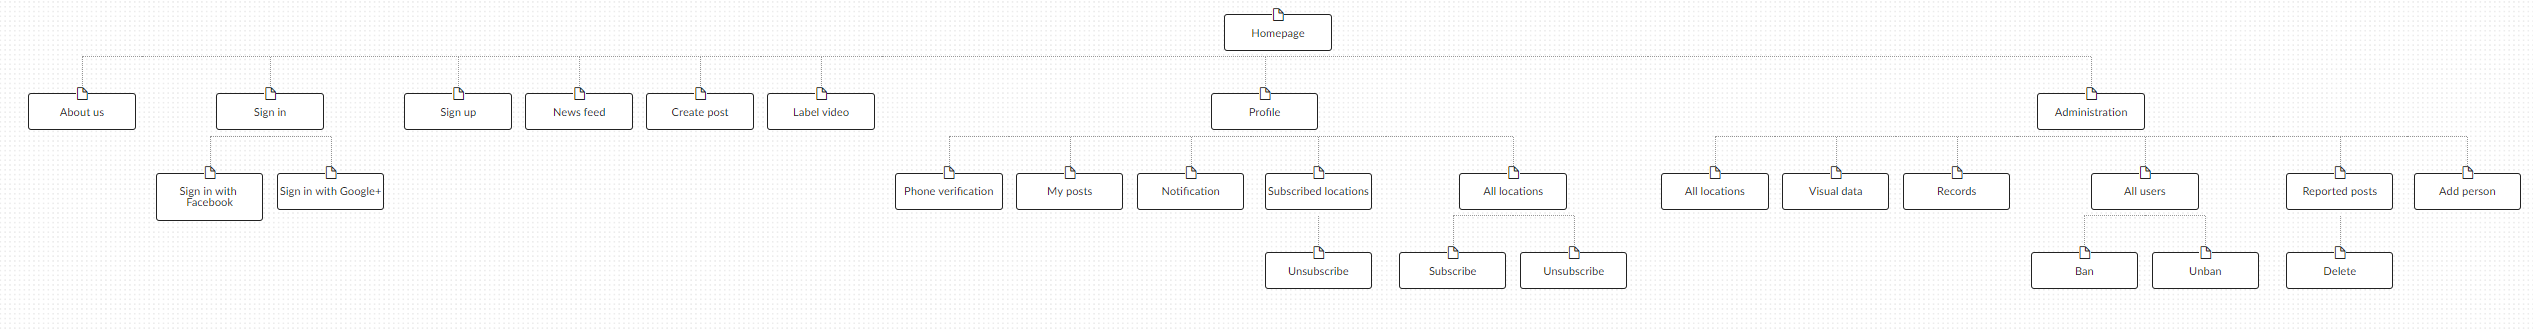
\includegraphics[width=0.16\columnwidth]{images/chap4/sitemap.png}
    \caption{Sitemap}
    \end{figure}
\end{center}
\subsubsection{Views}
\textbf{Header}
\\
Header is a navigation bar which is displayed in every views. Navigation bar only contains "About us", "Sign in", "Sign up" buttons by default.
\begin{center}
    \begin{figure}[H]
    \centering
    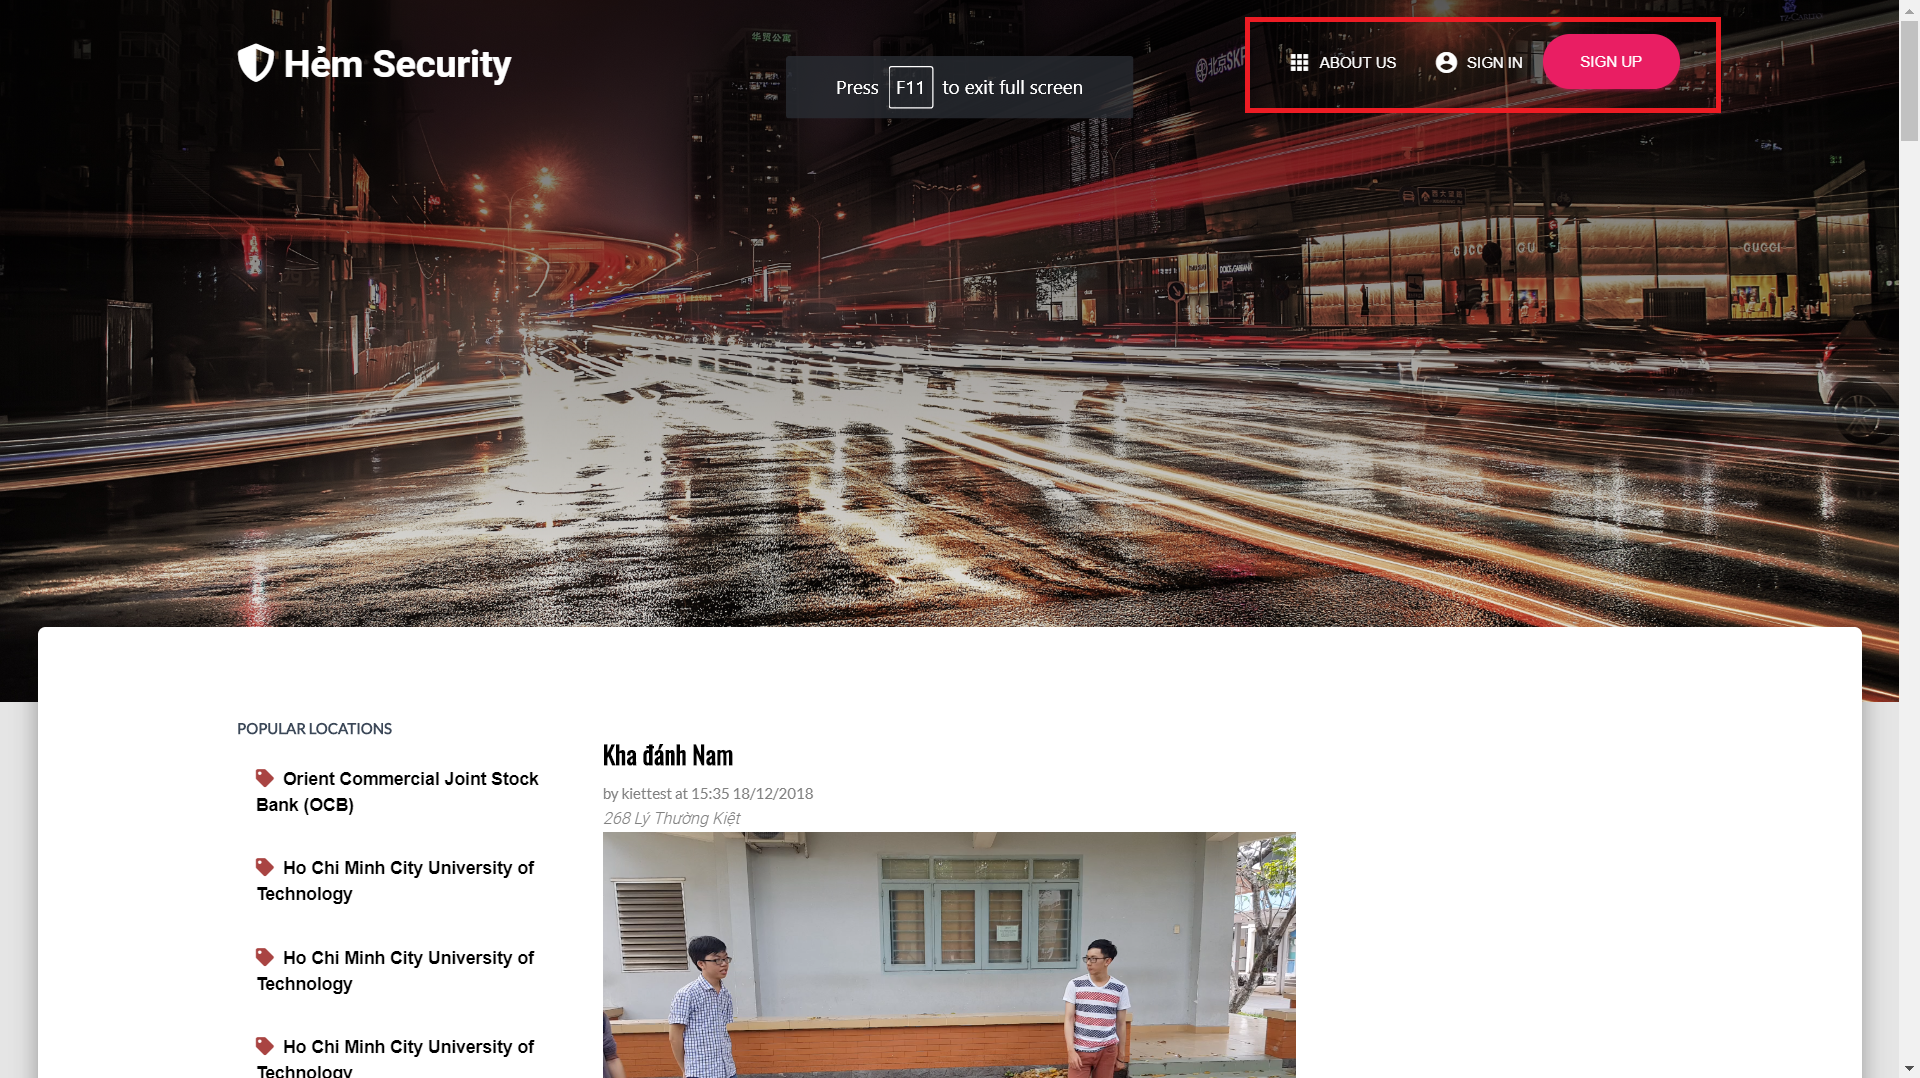
\includegraphics[width=1\columnwidth]{images/chap4/header_not_login.png}
    \caption{Default navigation bar.}
    \end{figure}
\end{center}

Logging in add additional buttons such as "Create post", "Label videos",  "Profile", "Log out" and a notification dropdown represented by a bell icon to the bar. In case of having unseen notifications, the bell icon will have an orange-red color.
\begin{center}
    \begin{figure}[H]
    \centering
    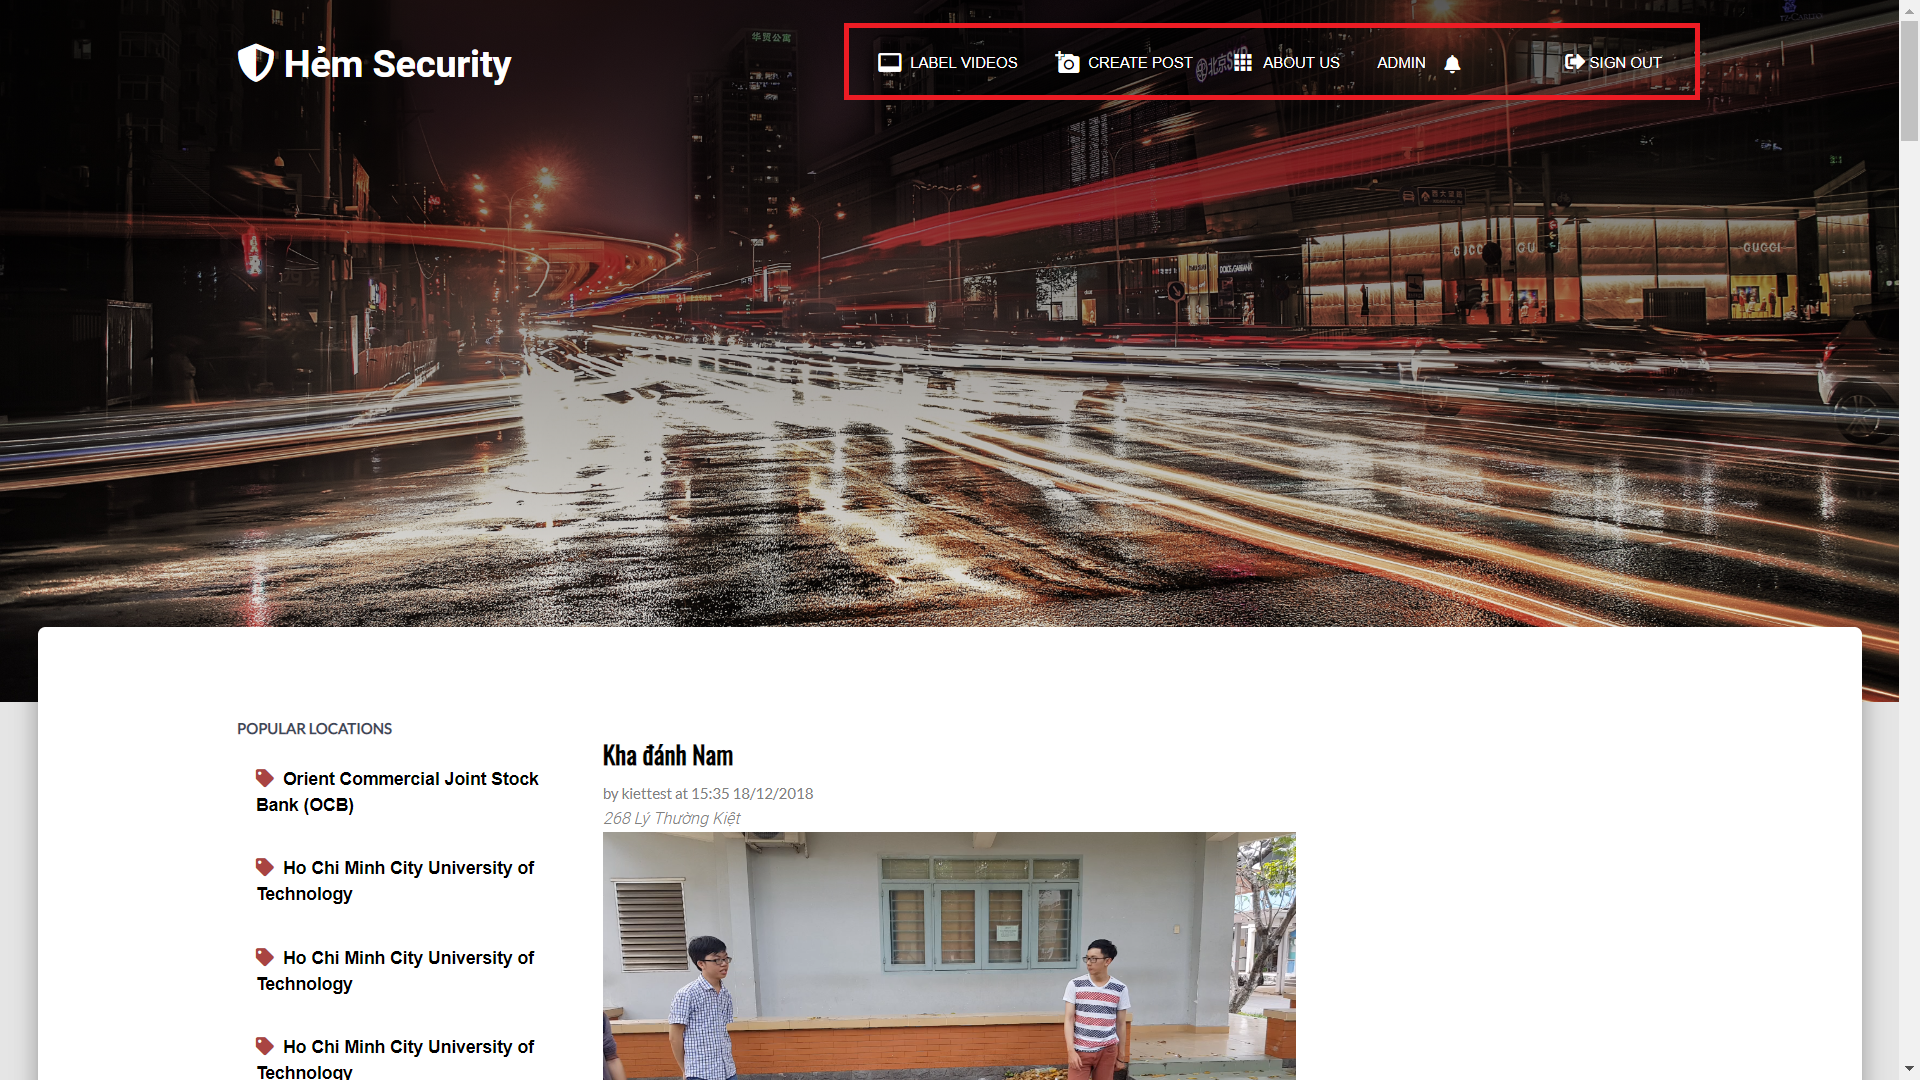
\includegraphics[width=1\columnwidth]{images/chap4/header.png}
    \caption{Navigation bar when logged in.}
    \end{figure}
\end{center}
\textbf{Homepage}
\\
News feed which are posts from everyone is visible in the middle of the homepage. A post is displayed with title, author, time, location and visual data. Additionally, there is a sidebar with popular locations. Clicking a location from the sidebar leads to another view that show only posts from that location. Blank space is reserved for advertising to earn income in the future.
\begin{center}
    \begin{figure}[H]
    \centering
    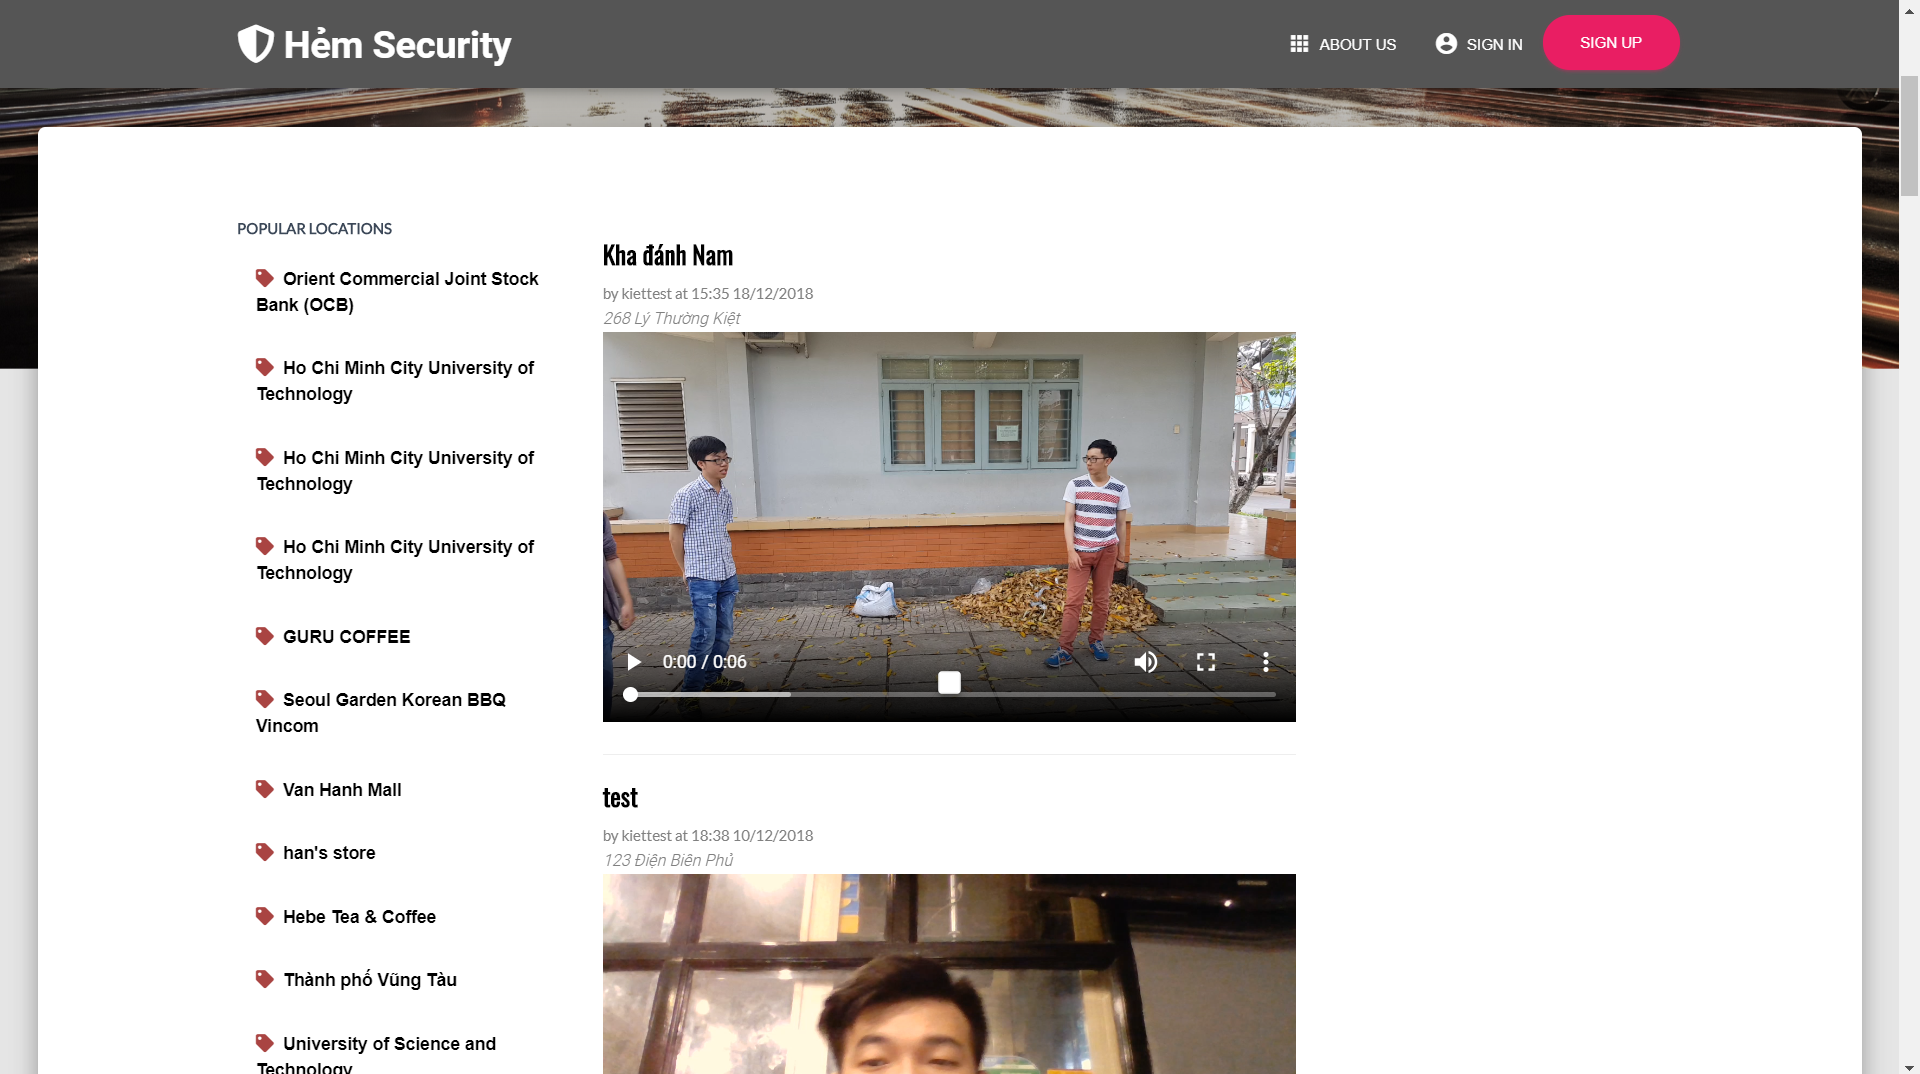
\includegraphics[width=1\columnwidth]{images/chap4/homepage.png}
    \end{figure}
\end{center}
\textbf{Sign in}
\\
Sign in form also has buttons for users to login with Google and Facebook account.
\begin{center}
    \begin{figure}[H]
    \centering
    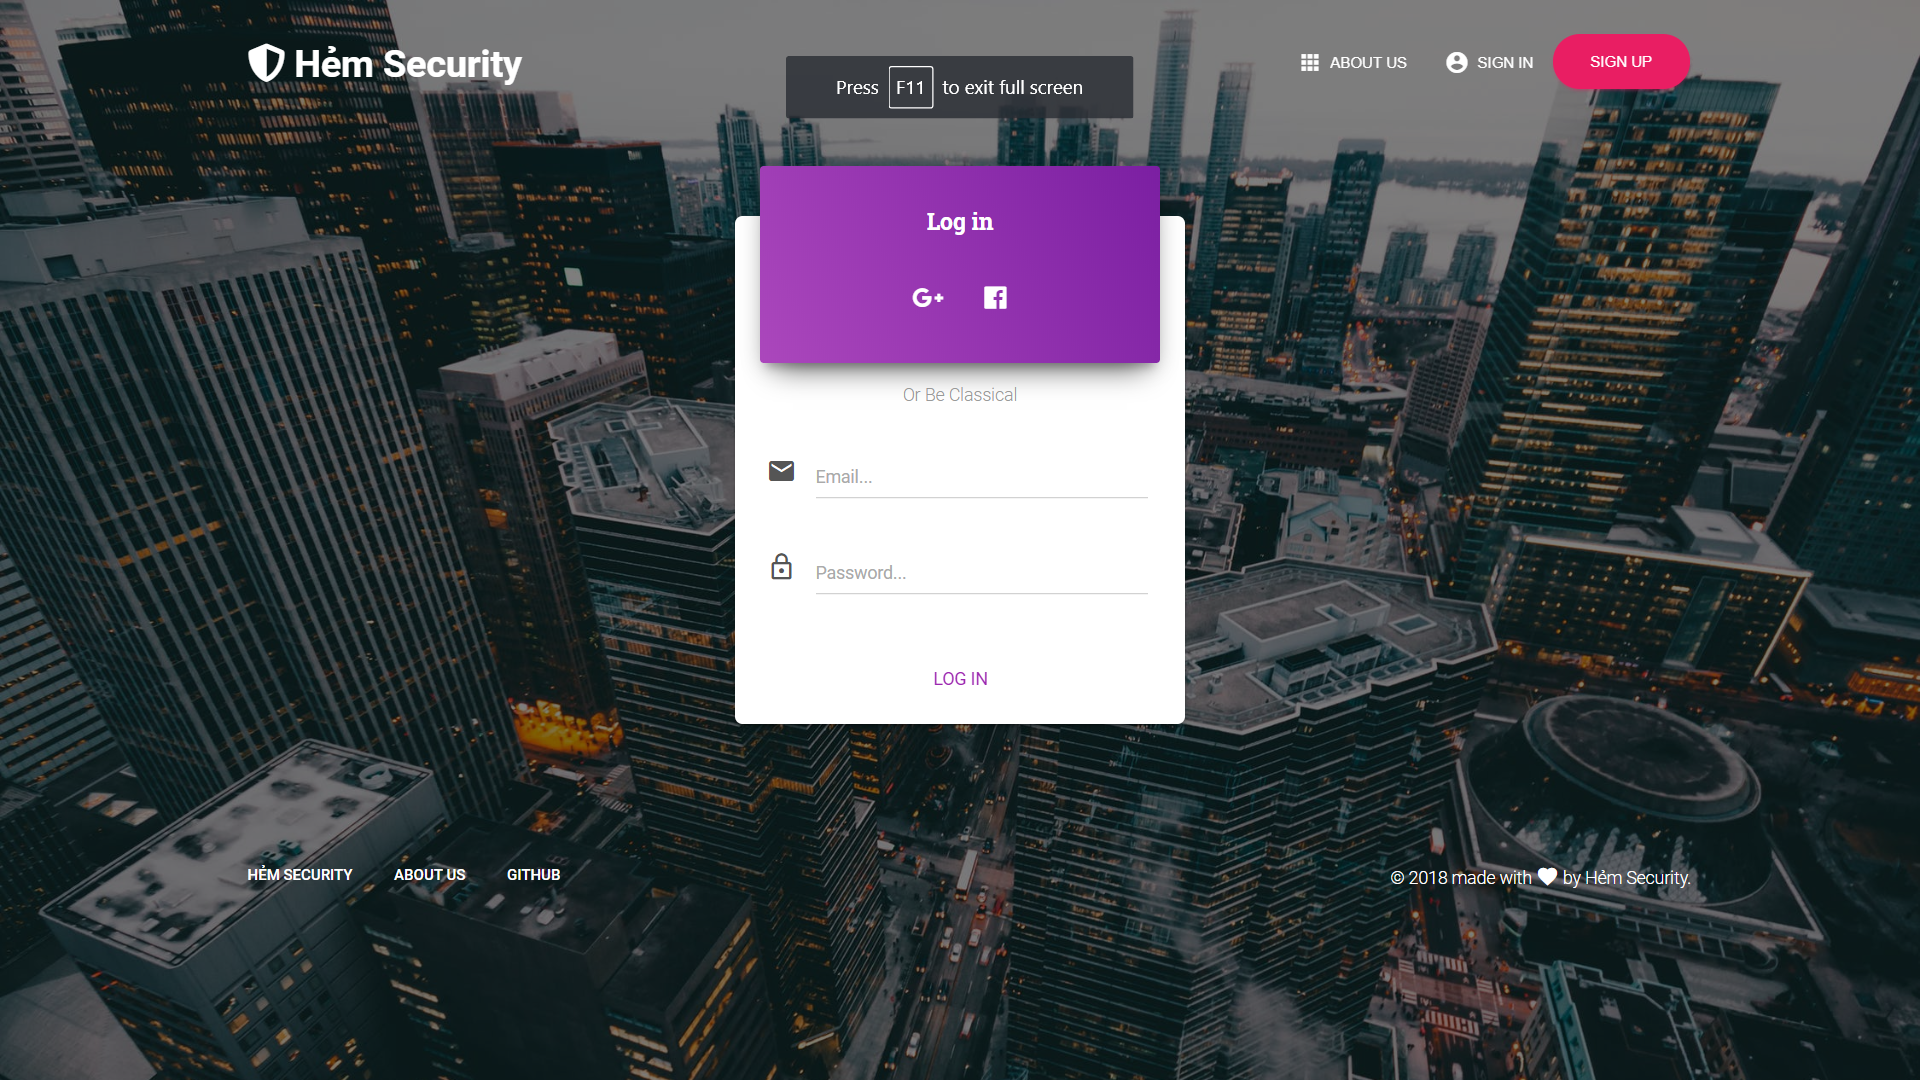
\includegraphics[width=1\columnwidth]{images/chap4/login_form.png}
    \end{figure}
\end{center}
\textbf{Sign up}
\\
Sign up form has general rules when using the website. Rule violation will result in banning violator's account.
\begin{center}
    \begin{figure}[H]
    \centering
    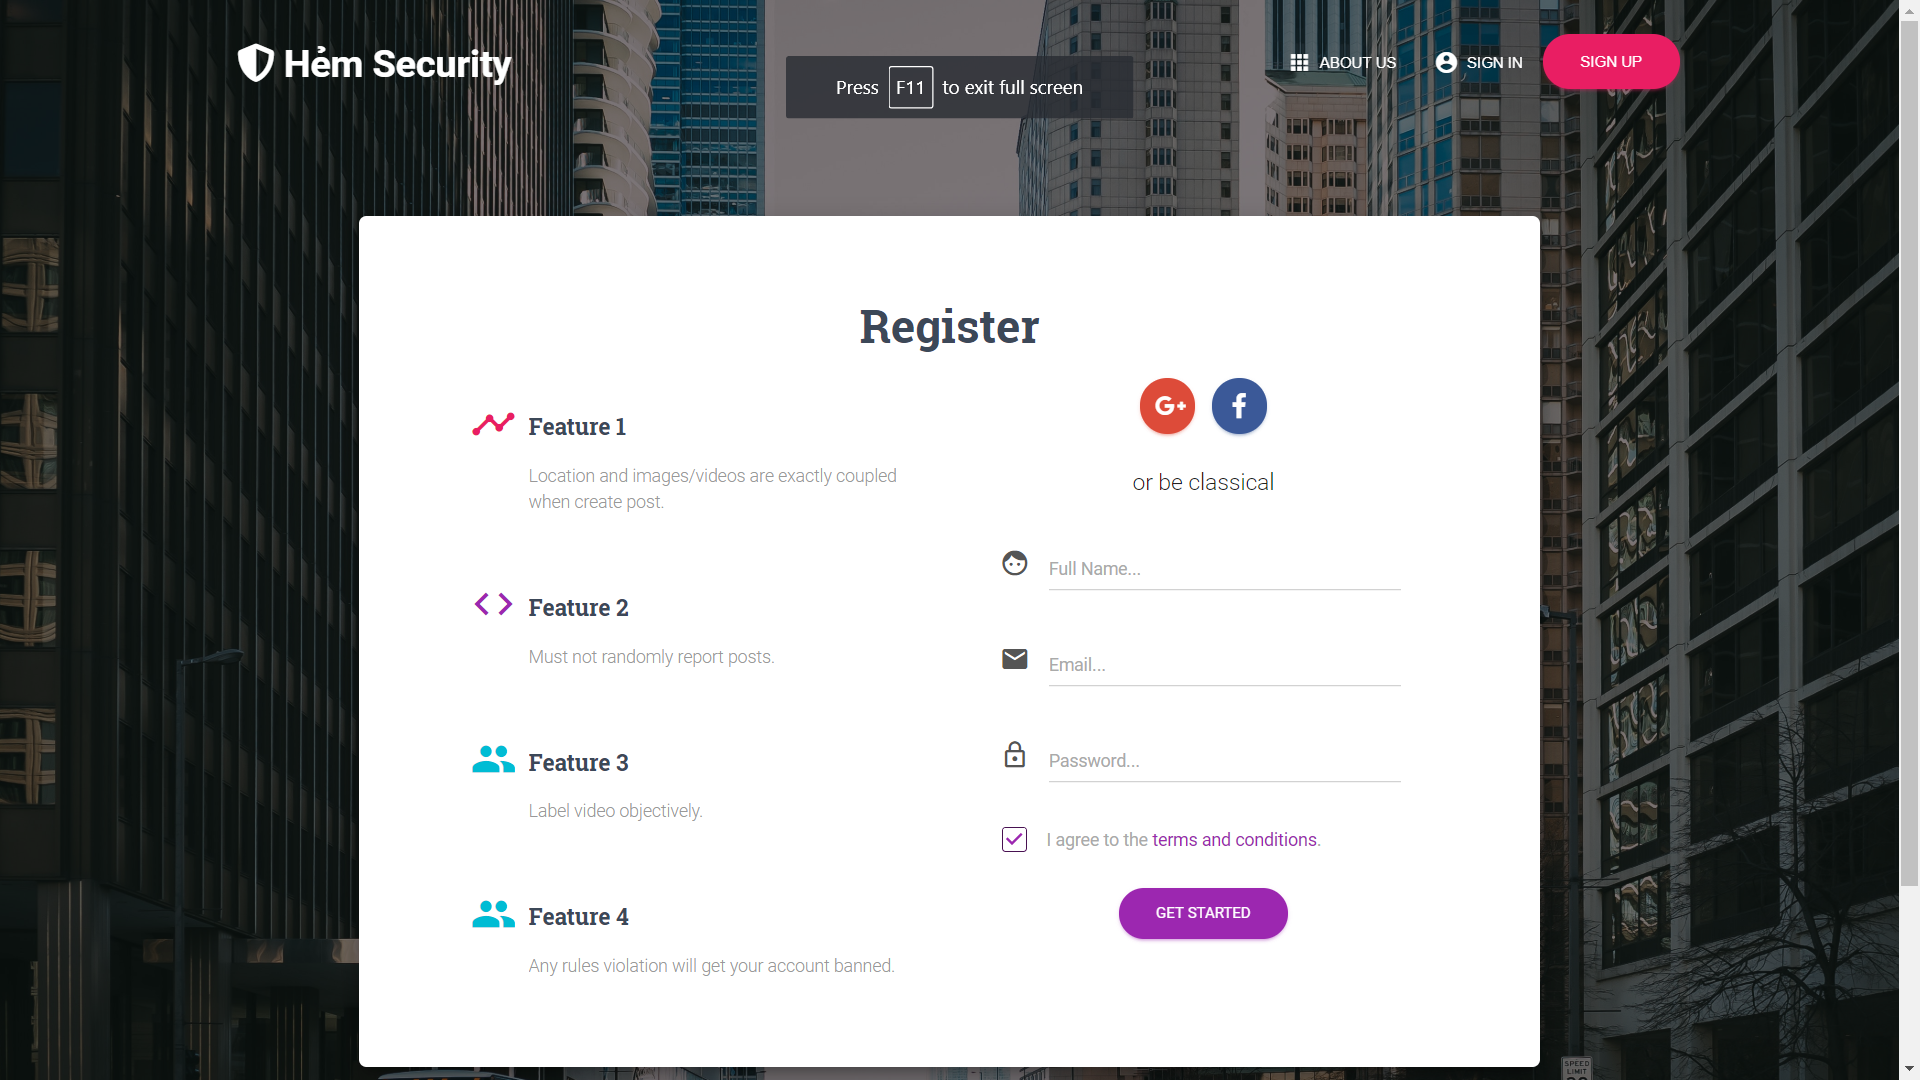
\includegraphics[width=1\columnwidth]{images/chap4/signup_form.png}
    \end{figure}
\end{center}
\textbf{Label video}
\\
Label video view contains a list of videos and two buttons "Suspicious" and "Not suspicious" for users to label. A user can only label a video once. Labeled videos are use to \textbf{xem lại}
\begin{center}
    \begin{figure}[H]
    \centering
    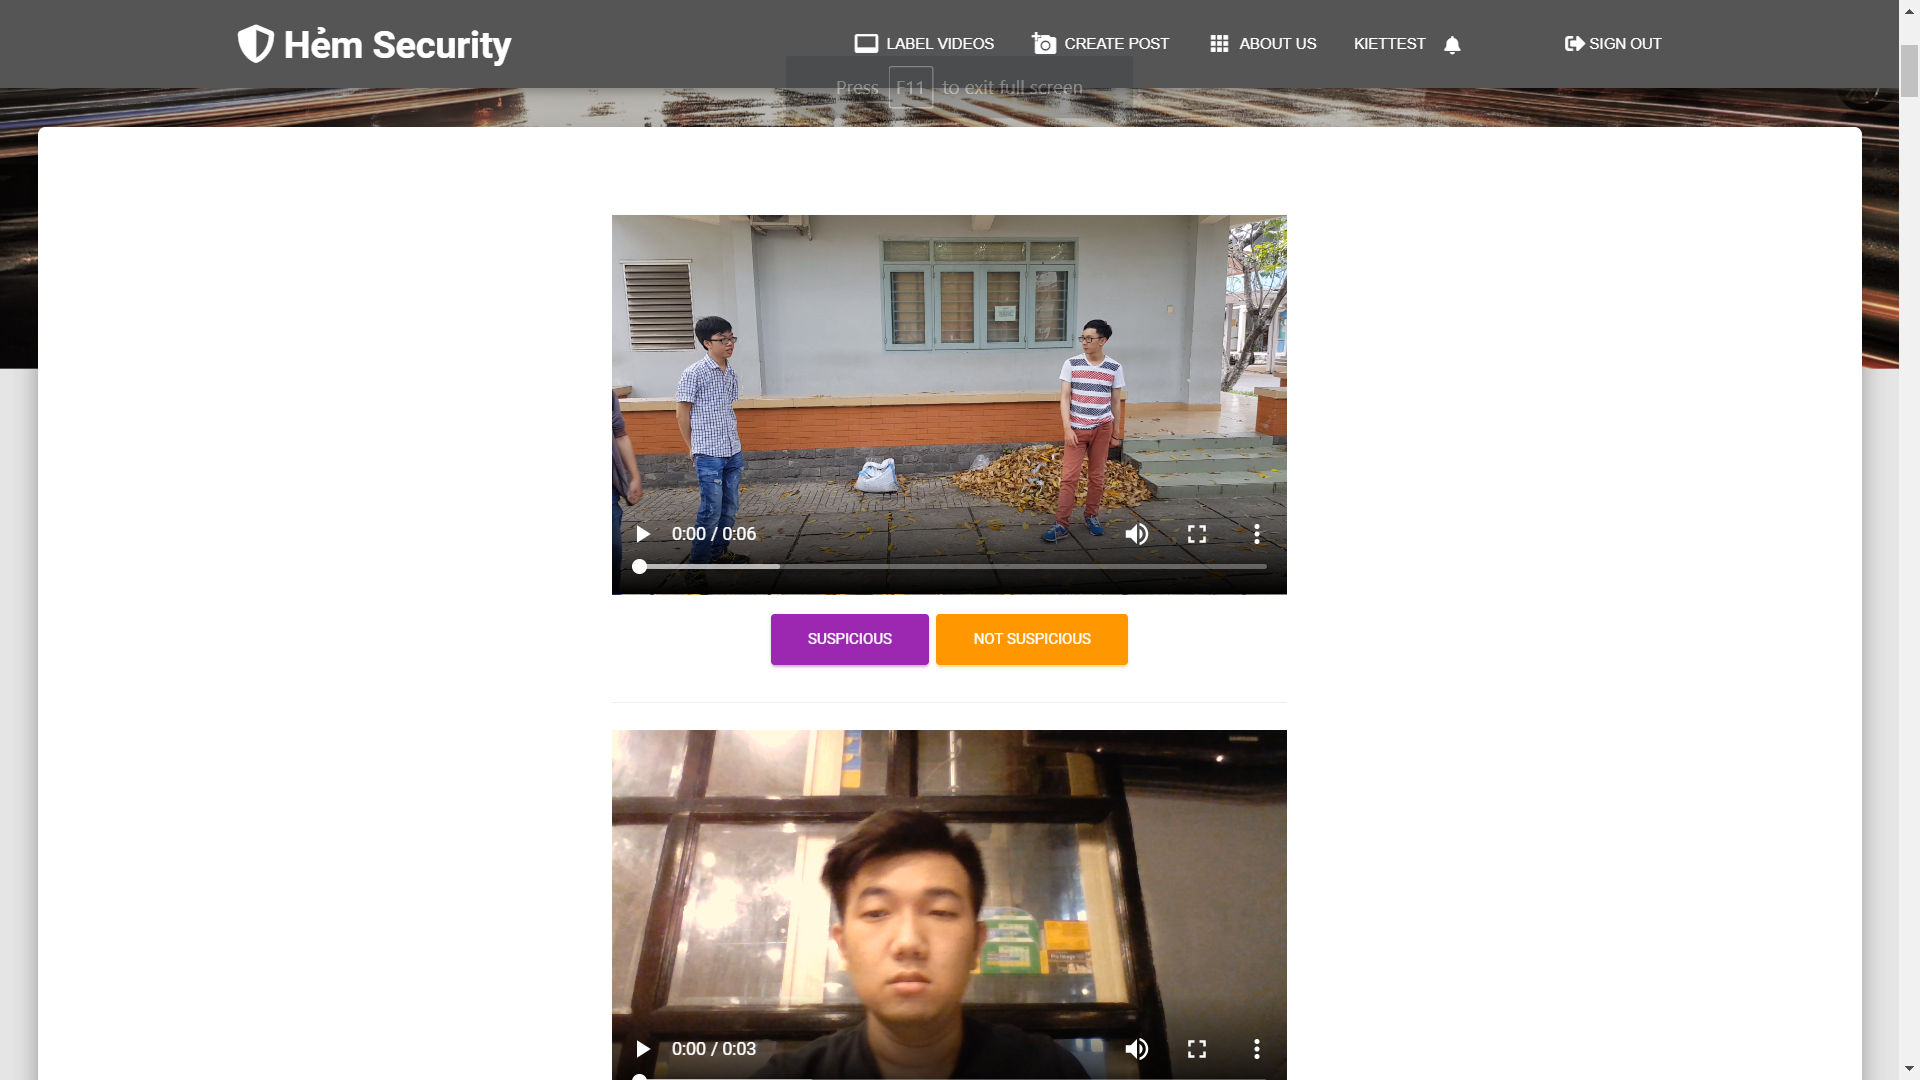
\includegraphics[width=1\columnwidth]{images/chap4/label_video.png}
    \end{figure}
\end{center}
\textbf{Create post}
\\
Create post form includes title, a file selector to select image/video, an embedded Google map to select location. After creating post, location of created post is available for other users to subscribe.

\begin{center}
    \begin{figure}[H]
    \centering
    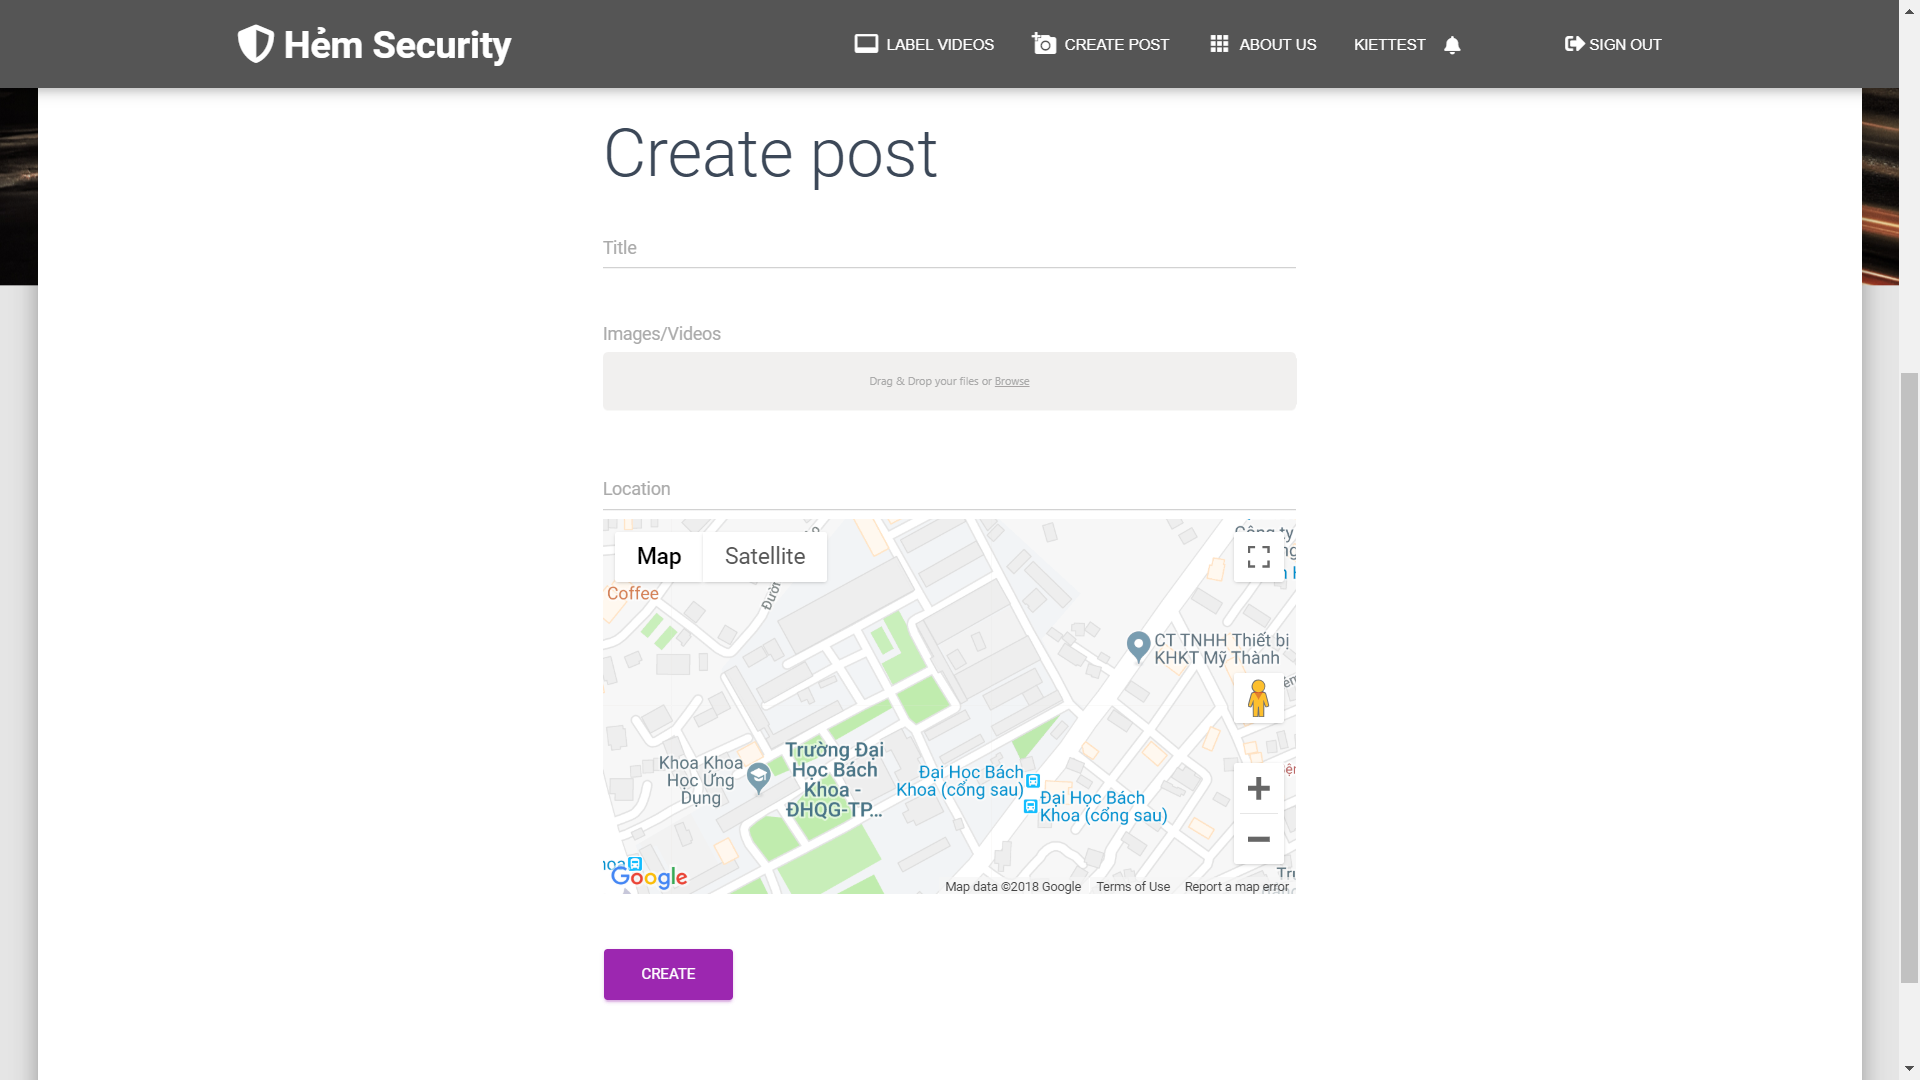
\includegraphics[width=1\columnwidth]{images/chap4/create_post.png}
    \end{figure}
\end{center}
\textbf{Profile}
\\
Profile view contains user's basic info and mobile phone field for verification. Besides, it also has 4 tabs:  
\begin{itemize}
\item My posts
\item Notifications
\item Subscribed locations: To unsubscribe a location.
\item All locations: To subscribe to a new location.
\end{itemize}
\begin{center}
    \begin{figure}[H]
    \centering
    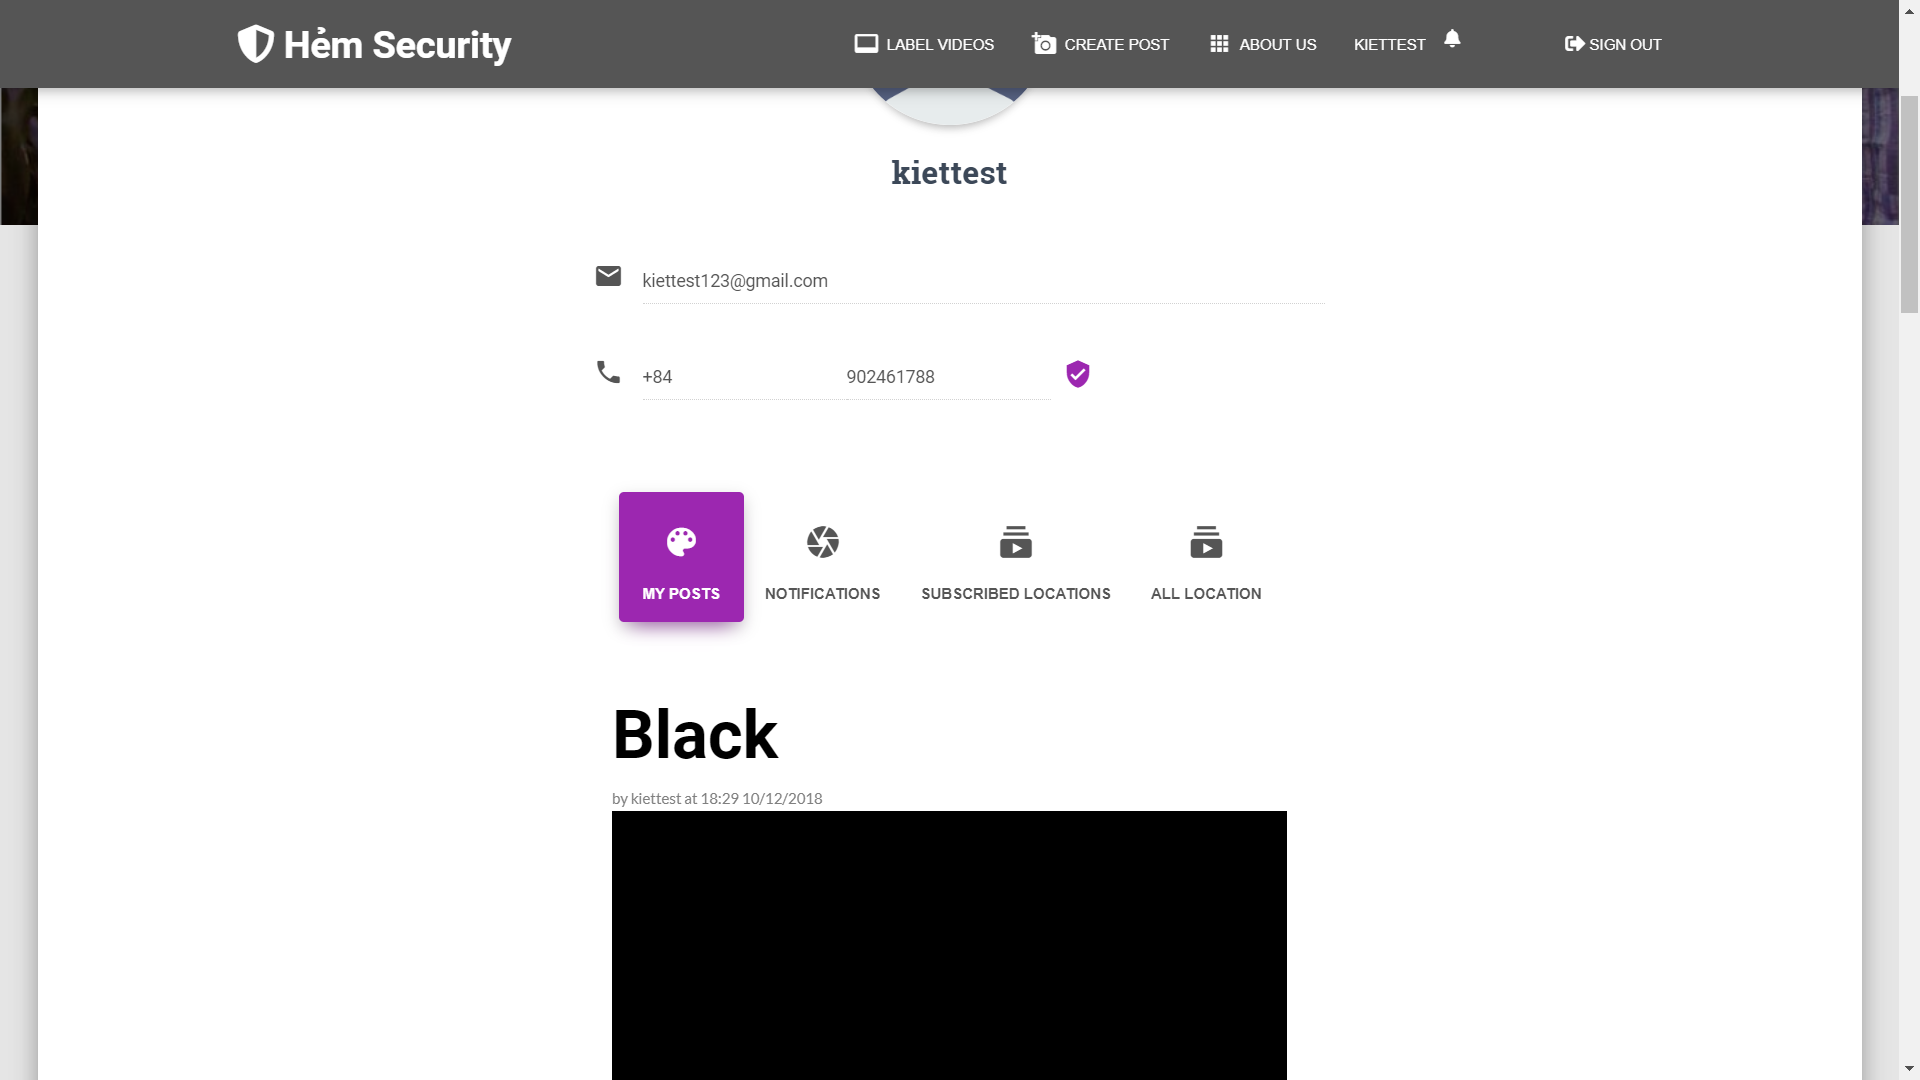
\includegraphics[width=1\columnwidth]{images/chap4/profile.png}
    \end{figure}
\end{center}
\textbf{Administration}
\\
Administration consists of 5 tabs:
\begin{itemize}
\item Locations
\item Visual data
\item Record: To look up an identified person's location history.
\item All users: To ban or unban a user.
\item Reported posts: To review reports and decide whether to delete post.
\end{itemize}
There is also an "Add person" button to add new person with name for system to identify in the future. An unidentified person is shown as "unknown".
\begin{center}
    \begin{figure}[H]
    \centering
    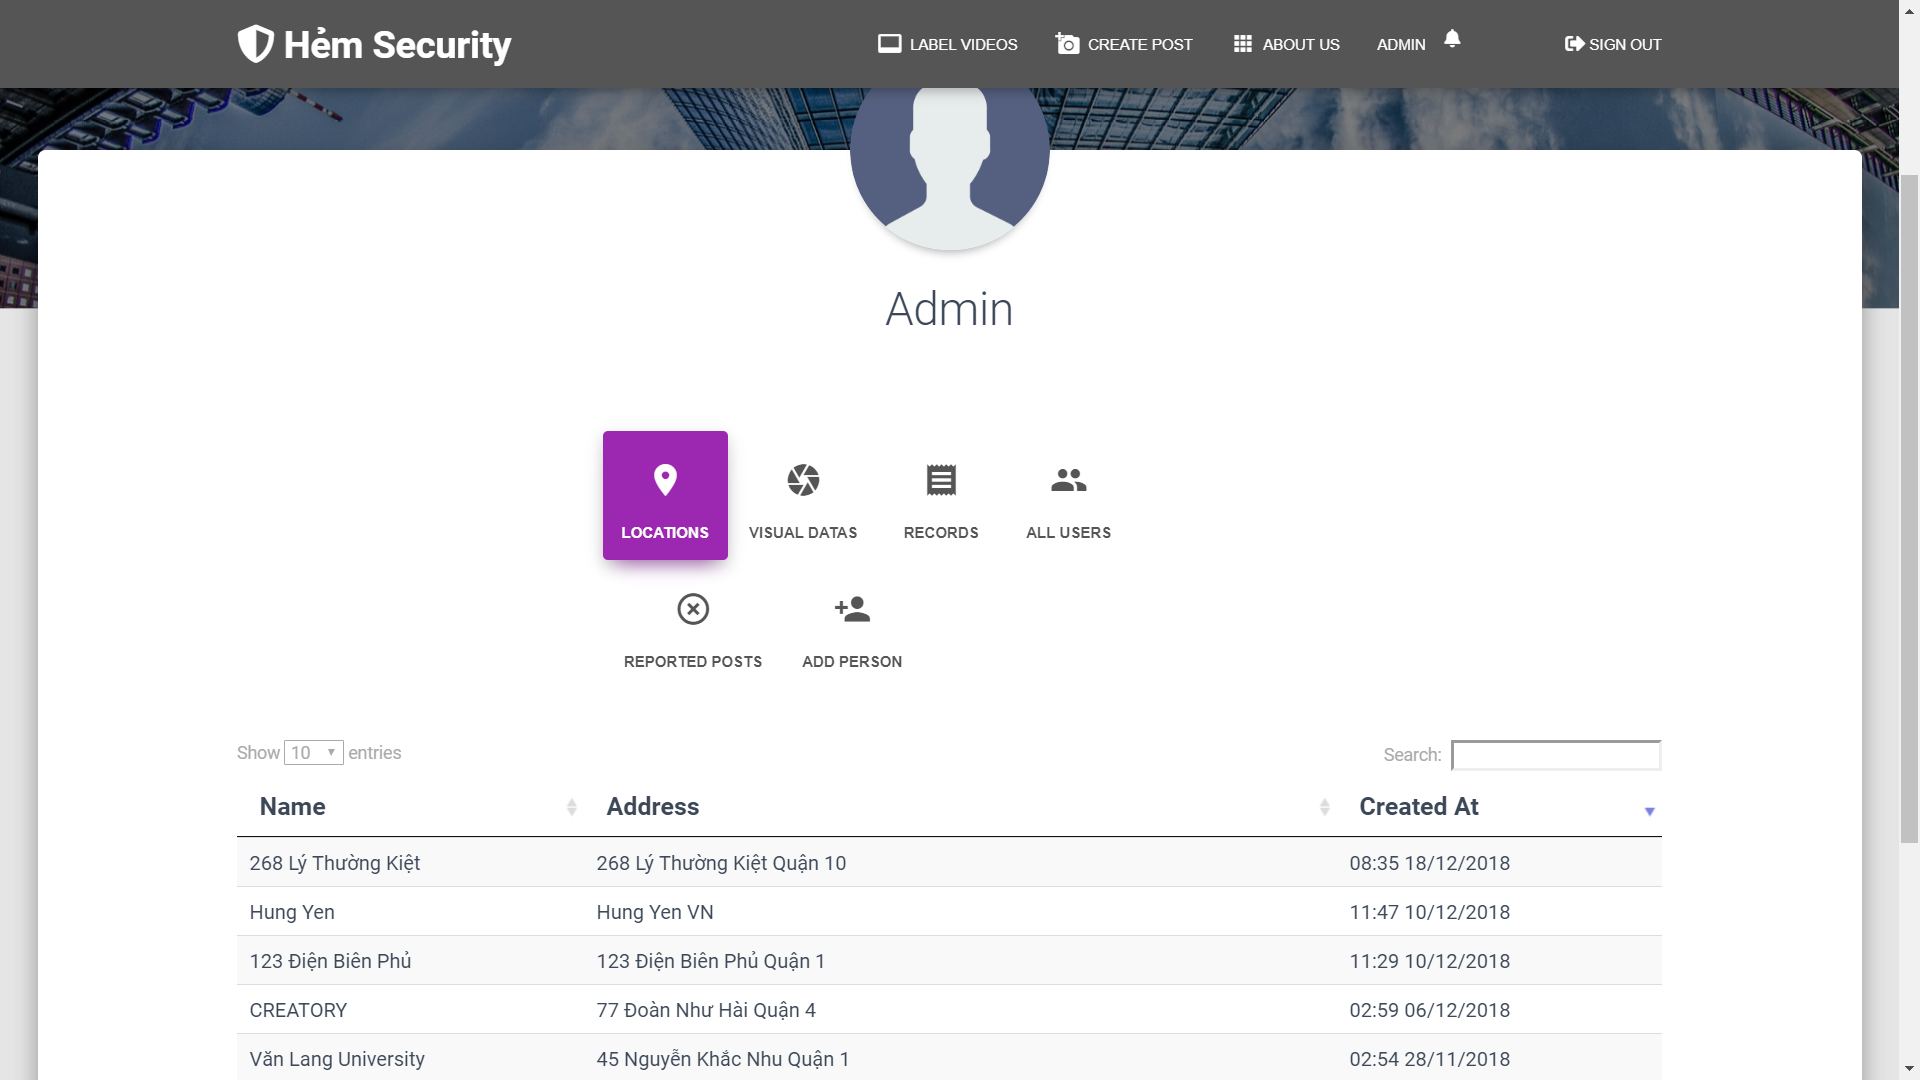
\includegraphics[width=1\columnwidth]{images/chap4/admin.png}
    \end{figure}
\end{center}
\subsection{Back-end}
In MVC pattern, the Controller receives user input, manipulates Model, and then responds to the user (cite). Following is the list of implemented controllers in this thesis.
\begin{itemize}
	\item Authentication Controller: manages the flow of user sign in and sign up. A user can choose either traditional or social login. With the classical way, the user has to provide his/her email and password. If the user prefers social login, this website currently supports sign in via Facebook and Google+.
	\item Dataset Collector: downloads dataset (a collection of labeled videos) as the input for the training process.
	\item Email Controller: One way to interact with users is sending emails. This controller sends email using SendGrid, an email delivery service.
	\item Face Controller: The core of Face Recognition Module is Microsoft Azure Face API, a cognitive service that provides algorithms for recognizing human faces in images (cite). Face Controller contains a bunch of function to request Microsoft Azure Face API.
	\item Identify Controller
	\item Location Controller: 
	\item Notification Controller
	\item Person Controller
	\item Post Controller
	\item Record Controller
	\item Upload Controller
	\item User Controller
	\item Visual Data Controller
	      
\end{itemize}
\section{Visual data analysis modules}
The project requires two systems for analysis: A face recognition system and a video classifier system. The facial recognition system takes pictures of human faces as input and returns their identification. The video classifier system analyzes videos to find out actions in them. The remaining of this section describes in detail about the two analysis system.
\subsection{Face recognition module}
The facial recognition module uses Microsoft Azure Face API as its core. “Azure Face API is a cognitive service that provides algorithms for detecting, recognizing, and analyzing human faces in images.” (cite + paraphase)
\begin{center}
    \begin{figure}[H]
    \centering
    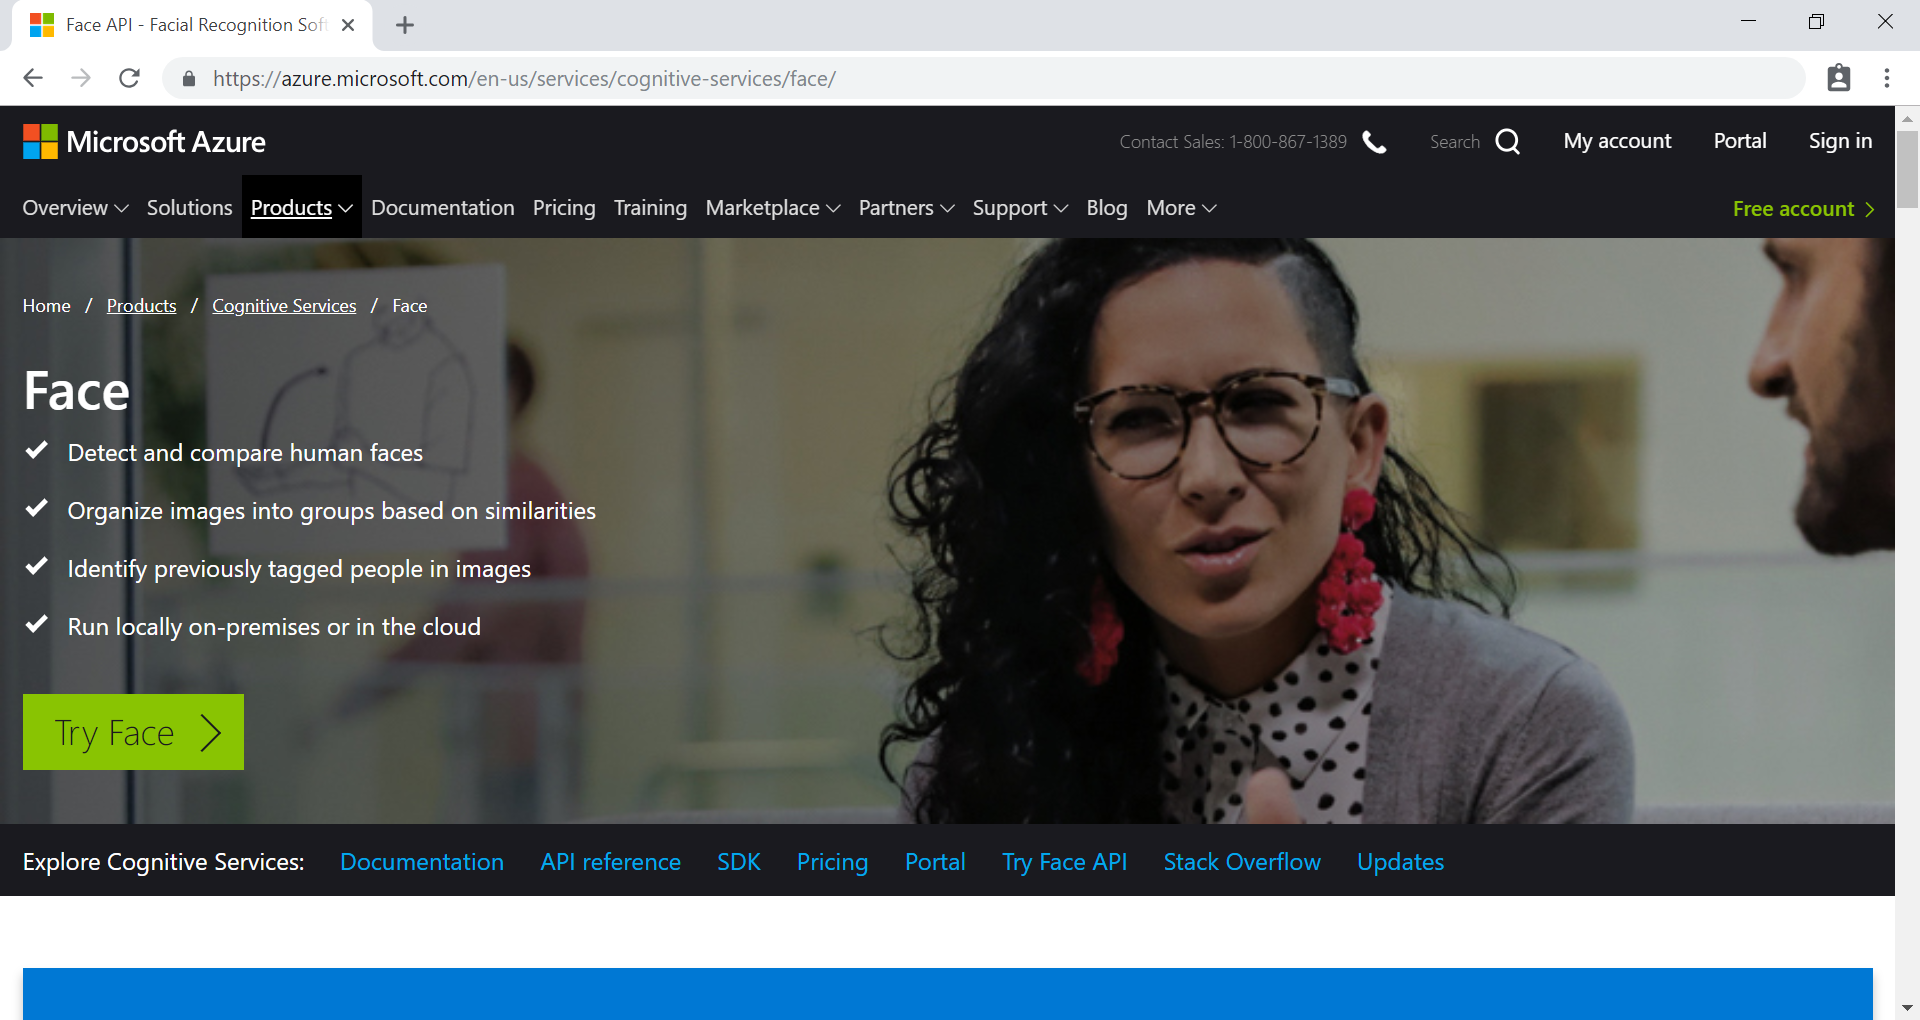
\includegraphics[width=1\columnwidth]{images/chap4/face-api-homepage.PNG}
    \caption{Microsoft Azure Face API hompage}
    \end{figure}
\end{center}
There is two way to use Azure Face Service: client Face SDK and Azure Face REST API. This thesis applies the second one. Both ways require a Face API subscription key in order to communicate with Microsoft Cognitive Server. This thesis applies the second one. The Face endpoint URL will be in the following format:
\begin{center}
\textit{https://[location].api.cognitive.microsoft.com/face/v1.0}
\end{center}
The location part will be replaced by the region of the subscription key (visit \href{https://westus.dev.cognitive.microsoft.com/docs/services/563879b61984550e40cbbe8d/operations/563879b61984550f30395236}{Face API docs} for a full list of all available regions). The Face API version currently is \textit{v1.0}.
Let take a look of some basic concepts for Face API from its \textit{Glossary} (cite):
\begin{itemize}
\item Face: is a result of a detected face, contains a unified identity (Face ID), face location in an image (Face Rectangle), and optional face attributes. Face ID will expire in 24 hours after detection call.
\item Persisted Face: similar to Face, but is persisted and will not expire.
\item Person: is an object which includes its identity (Person ID), a bunch of Persisted Face of that person, and other related data.
\item Person Group: is a set of Persons and is the unit of Identification. A Person Group must be specified in order to identify a face. Each face will be recognized independently. Before the Identification, the Person Group should be trained successfully.
\begin{center}
    \begin{figure}[H]
    \centering
    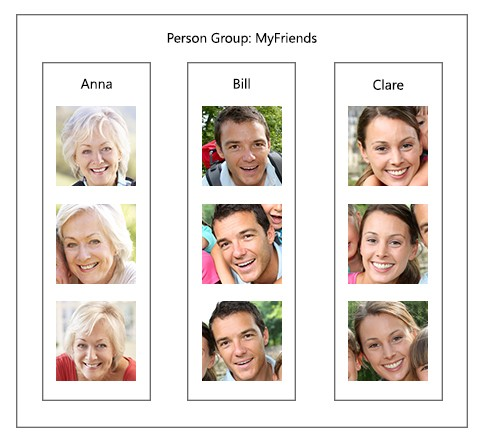
\includegraphics[width=1\columnwidth]{images/chap4/face-api-person-group.jpg}
    \caption{An example of Person Group}
    \end{figure}
\end{center}
\item Person Group - Create: This API will create a new Person Group with a unique Person Group ID, name, and user-provided user data (optional). This Person Group will contain uploaded person data, including face images and face recognition features.
\item Person Group - Train: In order to perform a face identification from a Person Group, that Person Group should be trained by calling this API. This API will pre-process the Person Group to ensure Identification performance.
\item Person Group Person – Create: This API will create a Person in a Person Group. It requires Person Name and Person Group ID. If a Person created successfully, it would return a new Person ID.
\item Person Group Person – Add Face: This API adds a Face image for a Person in a Person Group. It will return a Persisted Face ID after added. This Persisted Face will be used later for Identification or Verification request.
\item Face - Detect: This API accepts image (in binary data or image’s URL) as input, detects human faces in that picture; returns face coordinates and attributes. It can detect up to 64 faces in a photo, and best for frontal and near-frontal faces. Each detected face will be assigned a unique Face ID and will be used in Face - Identify.
\item Face - Identify: This API takes an array of Face ID (query faces), compute similarities with all Faces in that Person Group. After that, it returns identified results, which is a set of Persons with confidence.
\end{itemize}
\subsection{Video classifier module}
\subsubsection{Deploying the video classifier system}
After training the model and saving the weights, to use the model for prediction, this thesis proposes building an HTTP server and provide an API for other components to send requests and receive the result. \\
Flask framework is used to implement this HTTP server because of its fast performance and is written in Python which helps communication with Keras APIs easier.
\begin{center}
    \begin{figure}[H]
    \centering
    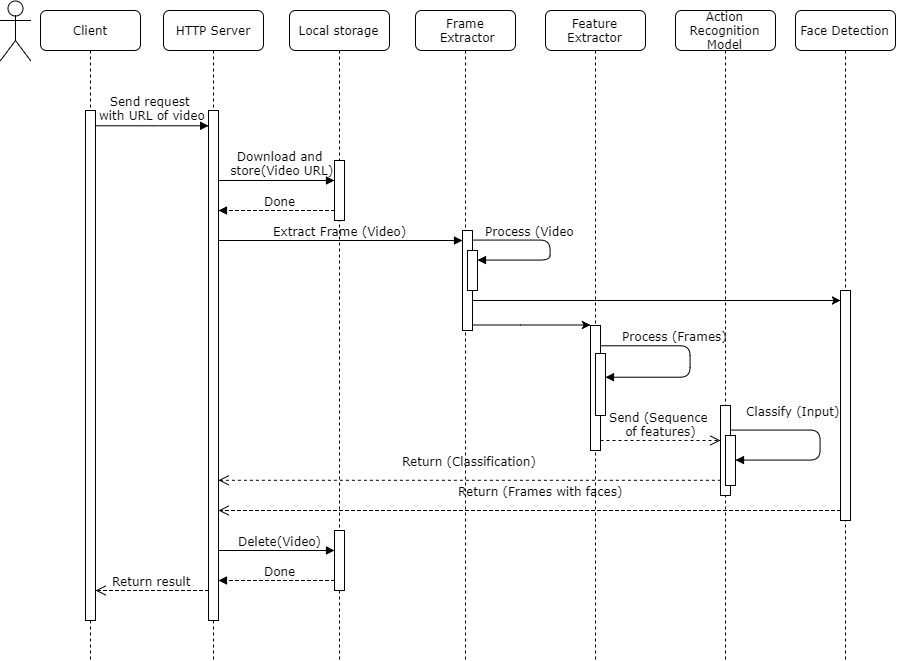
\includegraphics[width=1\columnwidth]{images/chap4/server_sequence.png}
    \caption{Sequence diagram of the HTTP server}
    \end{figure}
\end{center}
\subsubsection{Environment}
The classifier system was deployed using Google Compute Service. This service allows users to host virtual computers with customizable hardware for many purposes. The deployed server runs on the Ubuntu operating system because of its high performance, stability and its compatibility with deep learning codes. The server has the following hardware specification:

\begin{itemize}
	\item \textbf{CPU}:Xeon skylake 4 cores
	\item \textbf{RAM}:16GB
	\item \textbf{GPU}:K80 12GB
\end{itemize}
\textbf{NGINX} was used as the web server. It accepts any request from the default ports 80, 8080, then forward those request to a specified socket created by Gunicorn.\\
\textbf{Gunicorn} was used to serve the application. Gunicorn creates a socket so that web server could forward requests to, it then sends those request to the Python application. The Gunicorn process was set up as a system service so that it starts everytime the server boot up. Thec config file of this system service is in /etc/systemd/system/classifier-server.conf (Figure \ref{chap4:server_config}).
\begin{center}
    \begin{figure}[H]
    \centering
    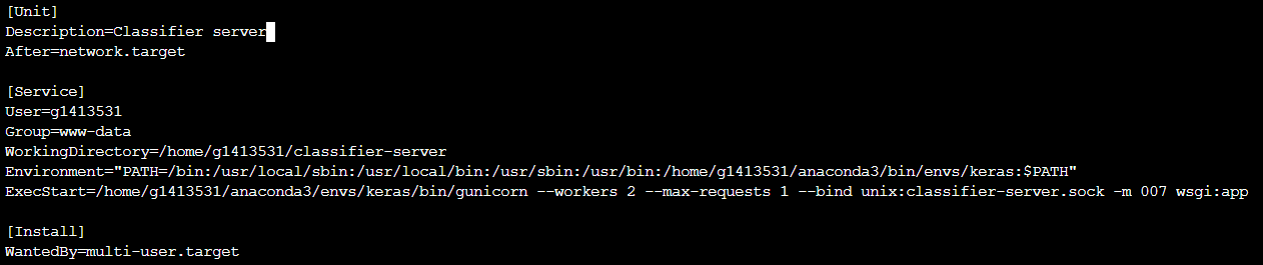
\includegraphics[width=1\columnwidth]{images/chap4/server_config.png}
	\caption{The config of Gunicorn system service. The \textbf{ExecStart} variable defines command to start this process. It spawn a maximum of 2 workers to serve requests, and each worker executes 1 requests before resetting. A socket named classifier-server.sock  is created to listen incoming request to this service.}   
	\label{chap4:server_config}
    \end{figure}
\end{center}

